\documentclass[11pt,oneside]{article}	%use"amsart"insteadof"article"forAMSLaTeXformat
\usepackage{geometry}		%Seegeometry.pdftolearnthelayoutoptions.Therearelots.
\geometry{letterpaper}		%...ora4paperora5paperor...
%\geometry{landscape}		%Activateforforrotatedpagegeometry
%\usepackage[parfill]{parskip}		%Activatetobeginparagraphswithanemptylineratherthananindent
\usepackage{graphicx}				%Usepdf,png,jpg,orepswithpdflatex;useepsinDVImode
								%TeXwillautomaticallyconverteps-->pdfinpdflatex		
\usepackage{amssymb}
\usepackage[colorlinks]{hyperref}

\usepackage{array}
\newcolumntype{P}[1]{>{\raggedright\arraybackslash}p{#1}}

%----macros begin---------------------------------------------------------------
\usepackage{color}
\usepackage{amsthm}
\usepackage{mathtools}

\def\conv{\mbox{\textrm{conv}\,}}
\def\aff{\mbox{\textrm{aff}\,}}
\def\E{\mathbb{E}}
\def\R{\mathbb{R}}
\def\Z{\mathbb{Z}}
\def\tex{\TeX}
\def\latex{\LaTeX}
\def\v#1{{\bf #1}}
\def\p#1{{\bf #1}}
\def\T#1{{\bf #1}}

\def\vet#1{{\left(\begin{array}{cccccccccccccccccccc}#1\end{array}\right)}}
\def\mat#1{{\left(\begin{array}{cccccccccccccccccccc}#1\end{array}\right)}}

\def\lin{\mbox{\rm lin}\,}
\def\aff{\mbox{\rm aff}\,}
\def\pos{\mbox{\rm pos}\,}
\def\cone{\mbox{\rm cone}\,}
\def\conv{\mbox{\rm conv}\,}
\newcommand{\homog}[0]{\mbox{\rm homog}\,}
\newcommand{\relint}[0]{\mbox{\rm relint}\,}

%----macros end-----------------------------------------------------------------

\title{ImagesToLARModel, a tool for creation of three-dimensional models from a stack of images}
\author{Danilo Salvati}
%\date{}							%Activatetodisplayagivendateornodate

\begin{document}
\maketitle
%\nonstopmode

\begin{abstract}
Here we will present a software for creating a three-dimensional model from a stack of images. This can be useful because of the simplicity of these type of representations. In particular a scope of use can be offered by medicine, where there is an enormous number of images but with very complex two-dimensional representations.\\

This work will use the LAR representation (\cite{cclar-proj:2013:00}) with the Julia language, because of its simplicity, showing how it can be used for quickly process image data.

\end{abstract}

\newpage
\tableofcontents
\newpage

%-------------------------------------------------------------------------------
%===============================================================================
\section{Introduction}\label{sec:intro}
%===============================================================================

This work has the aim to transform a two-dimensional representation of a model (based on a stack of images) into a three-dimensional representation based on the LAR schema. In particular, it will produce a single obj model which can be viewed with standard graphics softwares.\\

In the past were developed other softwares using same principles (see~\cite{paodcvjcadanda2015}). However, they were optimized for speed and cannot be able to accept huge amounts of data. With the rise of the big data era, we now have more and more data available for research purposes, so softwares must be able to deal with them. A typical hardware environment is based on a cluster of computers where computation can be distributed among a lot of different processes. However, as stated by \textit{Amdahl's law}, the speedup of a program using multiple processors is limited by the time needed for the sequential fraction of the program. So use of parallel techniques for dealing with big data is not important for time performance gain but for memory space gain. In fact, our biggest problem is lack of memory, due to model sizes. As a consequence, every parts of this software is written with the clear objective of minimizing memory usage at the cost of losing something in terms of time performance. So, for example, images will be converted in blocks determined by a grid size (see section~\ref{sec:ImagesConversion}) among different processes and different machines of the cluster

\begin{figure}[htb]
  \begin{center}
    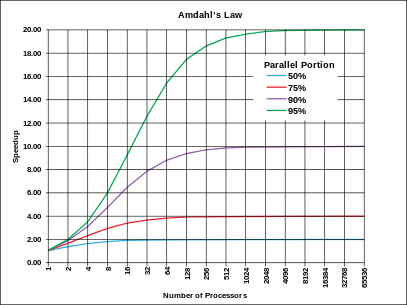
\includegraphics[width=8cm]{images/AmdahlsLaw.png}
  \end{center}
  \caption{Amdahl's law}
  \label{fig:Amdahl}
\end{figure}

\subsection{Why Julia}\label{sec:julia}
Ricordare che precedenti versioni erano in python\\
Semplicita\\
Efficienza\\
Capacita di realizzare programmi paralleli con poco sforzo\\
%-------------------------------------------------------------------------------


%-------------------------------------------------------------------------------
%===============================================================================
\section{Software structure}\label{sec:structure}
%===============================================================================

\subsection{Julia packages}\label{sec:juliaPkg}

This software will be distributed as a Julia Package. For the actual release (Julia 0.4) a package is a simple git project with the structure showed in figure~\ref{fig:julia-module}

\begin{figure}[htb]
  \begin{center}
    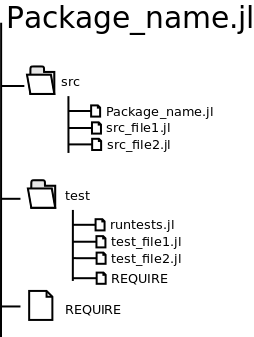
\includegraphics[width=4cm]{images/module-files.png}
  \end{center}
  \caption{Julia module structure}
  \label{fig:julia-module}
\end{figure}

Source code must be in folder \texttt{src}, while in \texttt{test} folder there are module tests with a \texttt{runtests.jl} for executing them and with a \texttt{REQUIRE} file for specifying tests dependencies. For listing dependencies for the entire project, there is another REQUIRE file in main folder. As an example in figure~\ref{fig:require-example} there is the REQUIRE file for \texttt{ImagesToLARModel.jl}.

\begin{figure}[htb]
  \begin{center}
    julia 0.3\\
    JSON\\
    Logging\\
    PyCall\\
    Images\\
    Colors\\
    Clustering
  \end{center}
  \caption{REQUIRE contents for \texttt{ImagesToLARModel.jl}}
  \label{fig:require-example}
\end{figure}

After creating this structure for a project it can be pushed on a git repository and installed on Julia systems. The usual installation procedure use this syntax:
\begin{quote}
 \texttt{Pkg.add("Package-name")}
\end{quote}

This will check for that package in METADATA.jl repository on github where there are all official Julia package. However it is also possible to install an unofficial package (on a public git repository) using this sintax:
\begin{quote}
 \texttt{Pkg.clone("git://repository-address.git")}
\end{quote}

This will install the package on your system with all the dependencies listed in REQUIRE file. 

\subsection{Architecture of ImagesToLARModel}\label{sec:architecture}

In previous section we have seen how to create a Julia package for distribute our application. Now we focus on the structure of our application. In \texttt{src} folder we can find the following modules:

\begin{description}
 \item \textbf{ImagesToLARModel.jl}: main module for the software, it takes input parameters and start images conversion
 \item \textbf{ImagesConversion.jl}: it is called by \texttt{ImagesToLARModel.jl} module and controls the entire conversion process calling all other modules
 \item \textbf{GenerateBorderMatrix.jl}: it generates the boundary operator for grid specified in input, saving it in a JSON file
 \item \textbf{PngStack2Array3dJulia.jl}: it is responsible of images loading and conversion into computable data
 \item \textbf{Lar2Julia.jl}: it contains a small subset of LAR functions written in Julia language
 \item \textbf{LARUtils.jl}: it contains utility functions for manipulation of LAR models
 \item \textbf{Smoother.jl}: it contains function for smoothing of LAR models
 \item \textbf{Model2Obj.jl}: it contains function that manipulates obj files
 \item \textbf{larcc.py}: python larcc module for boundary computation. In next releases of the software it will be rewritten in Julia language
\end{description}

In figure~\ref{fig:architecture} there is a simple schema of dependencies between modules.

\begin{figure}[htb]
  \begin{center}
    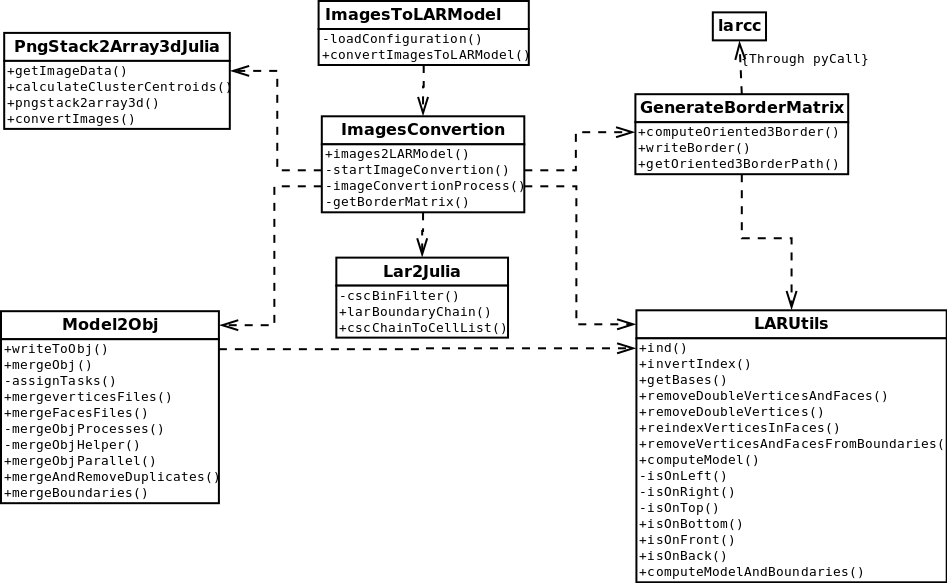
\includegraphics[width=16cm]{images/architecture.png}
  \end{center}
  \caption{Schema of module dependencies of ImagesToLARModel}
  \label{fig:architecture}
\end{figure}


Next sections of this document will explain in details all these modules showing also the code involved in conversion


%-------------------------------------------------------------------------------
%===============================================================================
\section{ImagesToLARModel}\label{sec:ImagesToLARModel}
%===============================================================================

This is the main module for the application; it takes the input data and start conversion calling \texttt{ImagesConversion.jl}.

\subsection{Calling modules}\label{sec:modules}

As we have already said, this first module has the responsibility of starting the conversion calling all other modules in the package. In Julia calling modules requires that they are in a path specified by \texttt{LOAD\_PATH} array.
So at the beginning of this module we need to add this line:

@D update load path
@{push!(LOAD_PATH, Pkg.dir("ImagesToLARModel/src"))
@}

\texttt{Pkg.dir()} function gives us the path of the Julia installation, so \texttt{Pkg.dir("ImagesToLARModel/src")} returns $``\langle Julia-path\rangle /ImagesToLARModel/src"$

After this line we can now import all modules defined here and export public functions:

@D modules import ImagesToLARModel
@{import JSON
import ImagesConversion

using Logging

export convertImagesToLARModel

@}

\subsection{Input loading}\label{sec:input}

Images conversion takes several parameters:

\begin{itemize}
 \item inputDirectory: The path of the directory containing the stack of images
 \item outputDirectory: The path of the directory containing the output
 \item bestImage: Image chosen for centroid computation (see section~\ref{sec:PngStack2Array3dJulia})
 \item nx, ny, nz: Sizes of the grid chosen for image segmentation (see section~\ref{sec:PngStack2Array3dJulia})
 \item DEBUG\_LEVEL: Debug level for Julia logger
 \item parallelMerge (experimental): Choose between sequential or parallel merge of files (see section~\ref{sec:Model2Obj})
\end{itemize}

Because of their number it has been realized a function for simply loading them from a JSON configuration file; this is the code:

@D load JSON configuration
@{function loadConfiguration(configurationFile)
  """
  load parameters from JSON file

  configurationFile: Path of the configuration file
  """

  configuration = JSON.parse(configurationFile)

  DEBUG_LEVELS = [DEBUG, INFO, WARNING, ERROR, CRITICAL]

  parallelMerge = false
  try
    if configuration["parallelMerge"] == "true"
      parallelMerge = true
    else
      parallelMerge = false
    end
  catch
  end

  return configuration["inputDirectory"], configuration["outputDirectory"],
	configuration["bestImage"],
        configuration["nx"], configuration["ny"], configuration["nz"],
        DEBUG_LEVELS[configuration["DEBUG_LEVEL"]],
        parallelMerge

end
@}

A valid JSON file has the following structure:
\begin{tabbing}
\{ \= \\
\>  ``inputDirectory": "Path of the input directory",\\
\>  ``outputDirectory": "Path of the output directory",\\
\>  ``bestImage": "Name of the best image (with extension) ",\\
\>  ``nx": x grid size,\\
\>  ``ny": y grid size,\\
\>  ``nz": border z,\\
\>  ``DEBUG\_LEVEL": julia Logging level (can be a number from 1 to 5)\\
\>  ``parallelMerge": "true" or "false" \\
\}\\
\end{tabbing}

For example, we can write:

\begin{tabbing}
\{ \= \\
\>  ``inputDirectory": ''/home/juser/IMAGES/``\\
\>  ``outputDirectory": ''/home/juser/OUTPUT/``,\\
\>  ``bestImage": ''0009.tiff``,\\
\>  ``nx": 2,\\
\>  ``ny": 2,\\
\>  ``nz": 2,\\
\>  ``DEBUG\_LEVEL": 2\\
\}\\
\end{tabbing}

As we can see, in a valid JSON configuration file DEBUG\_LEVEL can be a number from 1 to 5. Instead, when we explicitly define parameters, DEBUG\_LEVEL can only be one of the following Julia constants:

\begin{itemize}
 \item DEBUG
 \item INFO
 \item WARNING
 \item ERROR
 \item CRITICAL
\end{itemize}

\subsection{Starting conversion}\label{sec:input}

As we have already said, this module has the only responsibility to collect data input and starts other modules. These are the functions that start the process and the only exposed to the application users:

@D Start conversion from JSON file
@{function convertImagesToLARModel(configurationFile)
  """
  Start conversion of a stack of images into a 3D model
  loading parameters from a JSON configuration file

  configurationFile: Path of the configuration file
  """
  inputDirectory, outputDirectory, bestImage, nx, ny, nz,
      DEBUG_LEVEL, parallelMerge = loadConfiguration(open(configurationFile))
  convertImagesToLARModel(inputDirectory, outputDirectory, bestImage,
			nx, ny, nz, DEBUG_LEVEL, parallelMerge)
end
@}

@D Start manual conversion
@{function convertImagesToLARModel(inputDirectory, outputDirectory, bestImage,
                                 nx, ny, nz, DEBUG_LEVEL = INFO, parallelMerge = false)
  """
  Start conversion of a stack of images into a 3D model

  inputDirectory: Directory containing the stack of images
  outputDirectory: Directory containing the output
  bestImage: Image chosen for centroids computation
  nx, ny, nz: Border dimensions (Possibly the biggest power of two of images dimensions)
  DEBUG_LEVEL: Debug level for Julia logger. It can be one of the following:
    - DEBUG
    - INFO
    - WARNING
    - ERROR
    - CRITICAL
  """
  # Create output directory
  try
    mkpath(outputDirectory)
  catch
  end

  Logging.configure(level=DEBUG_LEVEL)
  ImagesConversion.images2LARModel(nx, ny, nz, bestImage,
	  inputDirectory, outputDirectory, parallelMerge)
end
@}

%===============================================================================
\section{PngStack2Array3dJulia}\label{sec:PngStack2Array3dJulia}
%===============================================================================

This module has the responsibility of convert a png image into an array of values
that will be passed to other modules

\subsection{Module imports}\label{sec:imports}
These are modules needed for this part of the package and the public functions exported

@D modules import PngStack2Array3dJulia
@{using Images # For loading png images
using Colors # For grayscale images
using PyCall
using Clustering
using Logging
@@pyimport scipy.ndimage as ndimage

NOISE_SHAPE_DETECT=10

export calculateClusterCentroids, pngstack2array3d, getImageData, convertImages
@}

We need \texttt{Images} and \texttt{Colors} packages for manipulating png images and \texttt{PyCall} for using Python functions for clustering and filtering images.
As a consequence, we need a python environment with \texttt{scipy} to be able to run the package

\subsection{Convert input to png}\label{sec:convertPNG}

First thing to do in our program is getting our input folder and convert the stack of images into png format. This process lets us to avoid managing an enormous variety of formats during computation, simplifying code used for transformation.\\

Conversion needs the following parameters:
\begin{itemize}
 \item inputPath: path of the folder containing the original images
 \item outputPath: path where we will save png images
 \item bestImage: name of the image chosen for centroids computing (see section~\ref{sec:centroids})
\end{itemize}

After conversion \textit{outputPath} will contain our png images and the function will return the new name chosen for the best image.\\

Now we can examine single parts of conversion process. First of all we need to specify a new name for images, keeping the right order between them; so we need to define a prefix based on number of images:

@D Define string prefix
@{imageFiles = readdir(inputPath)
numberOfImages = length(imageFiles)
outputPrefix = ""
for i in 1: length(string(numberOfImages)) - 1
  outputPrefix = string(outputPrefix,"0")
end @}
    
Next we need to open the single image doing the following operations:
\begin{enumerate}
 \item Open images using \texttt{Images} library (which relies on \texttt{ImageMagick}) and save them in greyscale png format 
 \item if one or both dimensions of the image are odd we need to remove one row (or column) of pixels to make it even. This will be more clear when we will introduce the grid for parallel computation (see section~\ref{sec:ImagesConversion})
\end{enumerate}

@D Greyscale conversion
@{rgb_img = convert(Image{ColorTypes.RGB}, img)
gray_img = convert(Image{ColorTypes.Gray}, rgb_img) @}
    
As we can see, we first need to convert image to RGB and then reconverting to greyscale. Without the RGB conversion these rows will return a stackoverflow error due to the presence of alpha channel


@D Image resizing
@{# resizing images if they do not have even dimensions
dim = size(img)
if(dim[1] % 2 != 0)
  debug("Image has odd x; resizing")
  xrange = 1: dim[1] - 1
else
  xrange = 1: dim[1]
end

if(dim[2] % 2 != 0)
  debug("Image has odd y; resizing")
  yrange = 1: dim[2] - 1
else
  yrange = 1: dim[2]
end

img = subim(gray_img, xrange, yrange) @}
    

Next we just have to search for the best image and add one image if they are odd (for same reasons we need even image dimensions)

@D Search for best image
@{# Searching the best image
if(imageFile == bestImage)
  newBestImage = string(outputPrefix[length(string(imageNumber)):end],
			    imageNumber,".png")
end
imageNumber += 1 @}
    
@D Add one image
@{# Adding another image if they are odd
if(numberOfImages % 2 != 0)
  debug("Odd images, adding one")  
  imageWidth, imageHeight = getImageData(string(outputPath, "/", newBestImage))
  
  if(imageWidth % 2 != 0)
    imageWidth -= 1
  end
  
  if(imageHeight % 2 != 0)
    imageHeight -= 1
  end  
  
  imArray = zeros(Uint8, imageWidth, imageHeight)
  img = grayim(imArray)
  outputFilename = string(outputPath, "/", 
		      outputPrefix[length(string(imageNumber)):end], imageNumber,".png")
  imwrite(img, outputFilename)
end @}


Fianlly we have to reduce noise on the image. The better choice is using a \textit{median filter} from package \texttt{scipy.ndimage} because it preserves better the edges of the image:

@D Reduce noise
@{# Denoising
imArray = raw(img)
imArray = ndimage.median_filter(imArray, NOISE_SHAPE_DETECT) @}

Where imArray is an array containing all raw data from images

Finally this is the code for the entire function:

@D Convert to png
@{function convertImages(inputPath, outputPath, bestImage)
  """
  Get all images contained in inputPath directory
  saving them in outputPath directory in png format.
  If images have one of two odd dimensions, they will be resized
  and if folder contains an odd number of images another one will be
  added

  inputPath: Directory containing input images
  outputPath: Temporary directory containing png images
  bestImage: Image chosen for centroids computation

  Returns the new name for the best image
  """

  @< Define string prefix @>
  
  newBestImage = ""
  imageNumber = 0
  for imageFile in imageFiles
    img = imread(string(inputPath, imageFile))
    @< Greyscale conversion @>
    @< Image resizing @>
    outputFilename = string(outputPath, outputPrefix[length(string(imageNumber)):end],
			      imageNumber,".png")
    imwrite(img, outputFilename)

    @< Search for best image @>
    @< Reduce noise @>
    
    img = grayim(imArray)
    imwrite(img, outputFilename)

  end

  @< Add one image @>

  return newBestImage
end
@}

\subsection{Getting data from a png}\label{sec:getData}

Now we need to load information data from png images. In particular we are interested in getting width and height of an image. As stated in~\cite{W3CPNG} document, a standard PNG file contains a \textit{signature} followed by a sequence of \textit{chunks} (each one with a specific type).\\

The signature always contain the following values:

\begin{quote}
 137 80 78 71 13 10 26 10
\end{quote}
   
This signature indicates that the remainder of the datastream contains a single PNG image, consisting of a series of chunks beginning with an \texttt{IHDR} chunk and ending with an \texttt{IEND} chunk. Every chunk is preceded by four bytes indicating its length.

As we are interested in width and height we need to parse the \texttt{IHDR} chunk. It is the first chunk in PNG datastream and its type field contains the decimal values:

\begin{quote}
 73 72 68 82
\end{quote}

The header also contains:\\

\begin{tabular}{l l}
  Width & 4 bytes\\
  Height & 4 bytes\\
  Bit depth & 1 bytes\\
  Color type & 1 byte\\
  Compression method & 1 byte\\
  Filter method & 1 byte\\
  Interlace method & 1 byte\\
\end{tabular}
\newline

So for reading width and height we need first 24 bytes; the first eight contain the signature, then we have four bytes for length, four bytes for the type field and eight bytes for information we are interested in. This is the code:

@D Get image data
@{function getImageData(imageFile)
  """
  Get width and height from a png image
  """

  input = open(imageFile, "r")
  data = readbytes(input, 24)
  
  if (convert(Array{Int},data[1:8]) != reshape([137 80 78 71 13 10 26 10],8))
    error("This is not a valid png image")
  end

  w = data[17:20]
  h = data[21:24]

  width = reinterpret(Int32, reverse(w))[1]
  height = reinterpret(Int32, reverse(h))[1]

  close(input)

  return width, height
end
@}

\subsection{Centroids computation}\label{sec:centroids}

As we have seen above, this package uses greyscale images for conversion into three-dimensional models and for next steps we need binary images so we can distinguish between the background and the model we want to represent. We can use clustering techniques for obtaining this result. First step is centroids calculation from a chosen image (this choice must be made from the user, because we cannot knowing in advance what is the best image for finding clusters).
Moreover we compute these centroids only for an image and then reuse them when we want to cluster all other images, saving processing time.\\
Actually we need only two centroids, because next steps should only recognize between background and foreground pixels.
This is the code used for centroid computation:

@D Centroid computation
@{function calculateClusterCentroids(path, image, numberOfClusters = 2)
  """
  Loads an image and calculate cluster centroids for segmentation

  path: Path of the image folder
  image: name of the image
  numberOfClusters: number of desidered clusters
  """
  imageFilename = string(path, image)

  img = imread(imageFilename) # Open png image with Julia Package

  imArray = raw(img)

  imageWidth = size(imArray)[1]
  imageHeight = size(imArray)[2]

  # Getting pixel values and saving them with another shape
  image3d = Array(Array{Uint8,2}, 0)

  # Inserting page on another list and reshaping
  push!(image3d, imArray)
  pixel = reshape(image3d[1], (imageWidth * imageHeight), 1)

  centroids = kmeans(convert(Array{Float64},transpose(pixel)), 2).centers

  return convert(Array{Uint8}, trunc(centroids))

end
@}

\subsection{Transform pixels into three-dimensional array}\label{sec:transformation}

Now we can study the most important part of this module, where images are converted into data usable by other modules for the creation of the three-dimensional model. The basic concept consists in transforming every single pixel in an integer value representing color, and then clustering them all using centroids computed earlier. So, we can obtain a matrix containing only two values (the two centroids) representing background and foreground of the image.\\
Now we will follow the code. This function uses four parameters

\begin{itemize}
 \item path: Path of the images directory
 \item minSlice: First image to read
 \item maxSlice: Last image to read
 \item centroids: Array containing centroids for clustering
\end{itemize}

For every image we want to transform in the interval [minSlice, maxSlice) we have to read it from disk and save pixel informations into a multidimensional Array:

@D Read raw data
@{img = imread(imageFilename) # Open png image with Julia Package
imArray = raw(img) # Putting pixel values into RAW 3d array @}

The \texttt{Images.jl} \texttt{raw} function, get all pixel values saving them in an Array. In Figure~\ref{fig:rawImage} we can see how the array will be like for a sample greyscale image.

\begin{figure}[htb] %  figure placement: here, top, bottom
   \centering
   
\includegraphics[width=0.27\linewidth]{images/grayscalesample.png}
   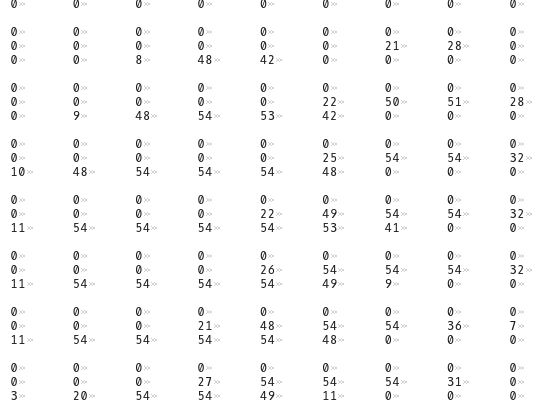
\includegraphics[width=0.47\linewidth]{images/imArraypart.png} \\
   
   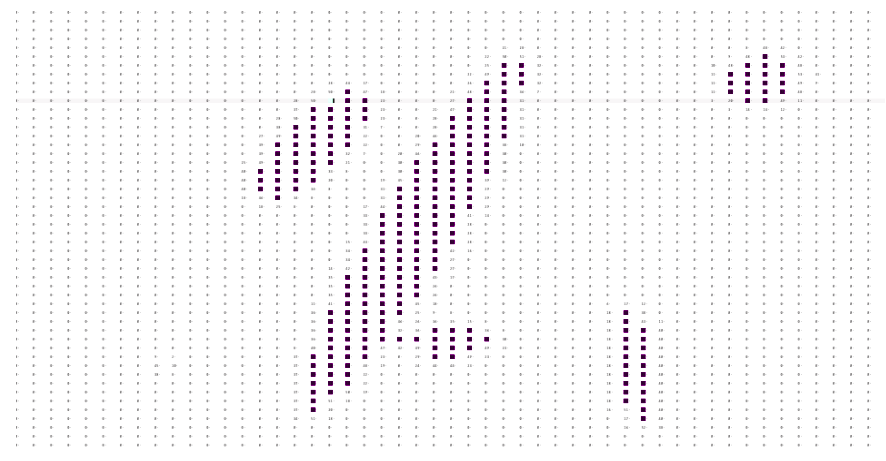
\includegraphics[width=0.67\linewidth]{images/imArrayfull.png} \hfill
   \caption{Reading raw data from image. (a) Original greyscale image (b) A view of raw data array (c) The entire raw data array with main color highlighted}
   \label{fig:rawImage}
\end{figure}

Finally we have to compute clusters obtaining images with only two values:

@D Clustering images
@{# Image Quantization
debug("page = ", page)
debug("image3d[page] dimensions: ", size(image3d[page])[1], "\t", size(image3d[page])[2])
pixel = reshape(image3d[page], size(image3d[page])[1] * size(image3d[page])[2] , 1)
kmeansResults = kmeans!(convert(Array{Float64},transpose(pixel)),
                convert(Array{Float64},centroids))

qnt = kmeansResults.assignments
centers = kmeansResults.centers
if(centers[1] == centers[2])
  # The image has only a value
  index = findmin([abs(centroids[1]-centers[1]),abs(centroids[2]-centers[1])])[2]
  qnt = fill(index, size(qnt))
end

# Reshaping quantization result
centers_idx = reshape(qnt, size(image3d[page],1), size(image3d[page],2))

# Inserting quantized values into 3d image array
tmp = Array(Uint8, size(image3d[page],1), size(image3d[page],2))

for j in 1:size(image3d[1],2)
  for i in 1:size(image3d[1],1)
    tmp[i,j] = centroids[centers_idx[i,j]]
  end
end

image3d[page] = tmp @}

\begin{figure}[htb] %  figure placement: here, top, bottom
   \centering
   
\includegraphics[width=0.30\linewidth]{images/grayscalesample.png} \hfill
   
\includegraphics[width=0.30\linewidth]{images/denoised.png} \hfill
   
\includegraphics[width=0.30\linewidth]{images/quantized.png} \hfill
   \caption{Image transformation. (a) Original greyscale image (b) Denoised image (c) Two-colors image}
   \label{fig:rawImage}
\end{figure}

We can see that sometimes the \texttt{Clustering.jl} library returns the same values for both centroid centers. This could happen when the images is completely empty or it has only colored pixels. So, we need to check this cases and fill the assignments array \texttt{qnt} with the right values based on the \texttt{centroids} parameter.

This is the complete code:

@D Pixel transformation
@{function pngstack2array3d(path, minSlice, maxSlice, centroids)
  """
  Import a stack of PNG images into a 3d array

  path: path of images directory
  minSlice and maxSlice: number of first and last slice
  centroids: centroids for image segmentation
  """

  # image3d contains all images values
  image3d = Array(Array{Uint8,2}, 0)

  debug("maxSlice = ", maxSlice, " minSlice = ", minSlice)
  files = readdir(path)

  for slice in minSlice : (maxSlice - 1)
    debug("slice = ", slice)
    imageFilename = string(path, files[slice + 1])
    debug("image name: ", imageFilename)
    @< Read raw data @>
    debug("imArray size: ", size(imArray))

    # Inserting page on another list and reshaping
    push!(image3d, imArray)

  end

  # Quantization
  for page in 1:length(image3d)

    @< Clustering images @>

  end

  return image3d
end
@}

%===============================================================================
\section{ImagesConversion}\label{sec:ImagesConversion}
%===============================================================================
Now we will study the most important module for this package: \texttt{ImagesConversion}. It has the responsibility of doing the entire conversion process delegating tasks to the other modules.

\subsection{General algorithm}\label{sec:generalAlgorithm}

Now we will examine, in a general way, the algorithm used for conversion from a two-dimensional to a three-dimensional representation of our biomedical models.\\
We have already seen in section~\ref{sec:PngStack2Array3dJulia} how to get information from a png image, obtaining arrays with only two values; one for the \textbf{background} color and one for \textbf{foreground} color. This is only the first step of the complete conversion process.\\

Now we focus only on a single image of the stack. Our two-dimensional representation, consists of pixels of two different colors (where only the one associated with foreground is significant); so we can obtain a three-dimensional representation simply replacing every foreground pixel with a small cube. Focusing on the entire stack of images, the full three-dimensional representation can be obtained simply overlapping all the image representations\\

This algorithm is very simple, however we does not considered problems concerning lack of memory. In fact, we could have images so big that we cannot build these models entirely in memory; moreover they would require a lot of CPU time for computation. A good solution to these problems consists in taking our representation based on images and divide according to a \textbf{grid}.\\

\begin{figure}[htb] %  figure placement: here, top, bottom
   \centering
   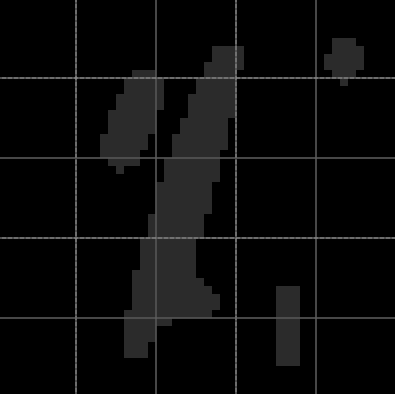
\includegraphics[width=0.45\linewidth]{images/imageGrid.png} \hfill
   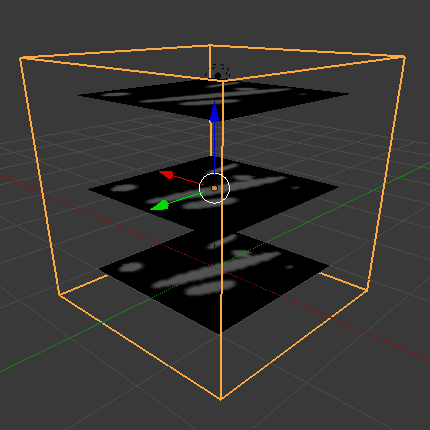
\includegraphics[width=0.45\linewidth]{images/imageGrid3d.png}
   \caption{The grid used for parallel computation (a) 2D grid on a single image (b) 3D grid for the stack of images}
   \label{fig:rawImage}
\end{figure}

So, instead of converting the entire model with a unique process, we can subdivide the input among a lot of processes, where every process will execute the conversion process on a small number of \textbf{blocks} according to the grid subdivision.\\

Summing up we can define the following terms, which will be used in next parts of this documentation:

\begin{itemize}
 \item \textbf{Grid:} It is the subdivision of the entire stack of images, with sizes defined by the user. They should be powers of two (for increasing performance during border matrix computation which we will see in section~\ref{sec:GenerateBorderMatrix})
 \item \textbf{Block:} It is a single cell of the grid
 \item \textbf{xBlock:} It is the x-coordinate of a block
 \item \textbf{yBlock:} It is the y-coordinate of a block
 \item \textbf{zBlock:} It is the z-coordinate of a block
\end{itemize}

\textit{xBlock} and \textit{yBlock} are defined on a single image, while \textit{zBlock} is defined on different images; in the code it will often be replaced by terms \textbf{StartImage} and \textbf{EndImage}, which indicate the first image and the last image of that block respectively.\\

In next subsections we will examine the conversion algorithm in detail, showing what happens for every block of the grid.

\subsection{Module imports}\label{sec:ImagesConversionImports}
These are modules needed for this part of the package and the public functions exported.

@D modules import ImagesConversion
@{import GenerateBorderMatrix
import PngStack2Array3dJulia
import Lar2Julia
import Model2Obj
import LARUtils
import Smoother

using Logging

export images2LARModel
@}

\subsection{Data preparation}\label{sec:ImagesConversionDataPreparation}
As a first thing, we will see how to prepare our data for conversion process. Firstly we need to convert input images to greyscale png; so we need to create a temporary directory for saving them.\\
Later, we need to compute the LAR boundary operator for finding boundaries of our cells (for the generation see section~\ref{sec:GenerateBorderMatrix}) getting width and height from our images.\\
Finally we can start conversion with all these parameters calling \texttt{startImageConversion} function, which will be explained in next subsection.

@D main function for ImagesConversion
@{function images2LARModel(nx, ny, nz, bestImage,
			inputDirectory, outputDirectory, parallelMerge)
  """
  Convert a stack of images into a 3d model
  """

  info("Starting model creation")

  numberOfClusters = 2 # Number of clusters for
                       # images segmentation

  info("Moving images into temp directory")
  try
    mkdir(string(outputDirectory, "TEMP"))
  catch
  end

  tempDirectory = string(outputDirectory,"TEMP/")

  newBestImage = PngStack2Array3dJulia.convertImages(inputDirectory, tempDirectory,
							bestImage)

  imageWidth, imageHeight = PngStack2Array3dJulia.getImageData(
				      string(tempDirectory,newBestImage))
  imageDepth = length(readdir(tempDirectory))

  # Computing border matrix
  info("Computing border matrix")
  try
    mkdir(string(outputDirectory, "BORDERS"))
  catch
  end
  borderFilename = GenerateBorderMatrix.getOriented3BorderPath(
					string(outputDirectory, "BORDERS"), nx, ny, nz)

  # Starting images conversion and border computation
  info("Starting images conversion")
  startImageConversion(tempDirectory, newBestImage, outputDirectory, borderFilename,
                       imageHeight, imageWidth, imageDepth,
                       nx, ny, nz,
                       numberOfClusters, parallelMerge)

end
@}

\subsection{Conversion pipeline}\label{sec:conversionpipeline}

Now we can see how conversion of images works. In section~\ref{sec:generalAlgorithm} we have seen how to execute the single conversion of a pixel into a voxel using our grid for parallel computation. However, with that algorithm, we obtain models with internal boundaries between blocks and with squared edge. So we need to create a \textbf{conversion pipeline} which will progressively refine our models. In Figure~\ref{fig:Pipeline} there are the steps used for our conversion

\begin{figure}[htb] %  figure placement: here, top, bottom
   \centering
   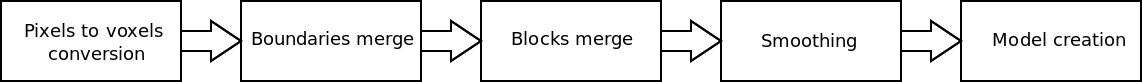
\includegraphics[width=1.10\linewidth]{images/Pipeline.png}
   \caption{Images conversion pipeline}
   \label{fig:Pipeline}
\end{figure}

Every single step of the pipeline, is executed in parallel for every block of the grid; so we need a general purpose function for blocks iteration which will take as a parameter a function that will execute it. So we can define the \texttt{iterateOnBlocks} function which takes the following parameters:
\begin{itemize}
 \item \textbf{inputDirectory}: Directory which contains input files for the process function
 \item \textbf{imageHeight, imageWidth, imageDepth}: Sizes of the stack of images
 \item \textbf{imageDx, imageDy, imageDz}: Sizes of the grid
 \item \textbf{processFunction}: Function that contains instructions for execution of a single step of the pipeline for a single block
 \item \textbf{outputDirectory}: Directory which will contains the output
 \item \textbf{centroids}: Centroids from the best image
 \item \textbf{boundaryMat}: Boundary operator for the chosen grid
\end{itemize}

This function will iterate on all blocks of the image grid executing the process function, which will be different for every pipeline step. This is the code used:

@D parallel block iteration
@{function iterateOnBlocks(inputDirectory,
                         imageHeight, imageWidth, imageDepth,
                         imageDx, imageDy, imageDz,
                         processFunction, outputDirectory,
                         centroidsCalc, boundaryMat)
  """
  Simple function that iterates on blocks for executing
  a task described by a processFunction

  inputDirectory: Directory which contains input files for the process function
  imageHeight, imageWidth, imageDepth: Images sizes
  imageDx, imageDy, imageDz: Sizes of cells grid
  processFunction: Function that will be executed on a separate task on
  the entire z-Block
  outputDirectory: Directory which will contains the output
  centroidsCalc: Centroids from the best image
  boundaryMat: Boundary operator for the chosen grid
  """

  beginImageStack = 0
  endImage = beginImageStack

  tasks = Array(RemoteRef, 0)
  for zBlock in 0:(imageDepth / imageDz - 1)
    startImage = endImage
    endImage = startImage + imageDz
    task = @@spawn processFunction(inputDirectory,
				   startImage, endImage,
                                   imageDx, imageDy,
                                   imageWidth, imageHeight,
                                   outputDirectory,
                                   centroidsCalc, boundaryMat)                                  
    push!(tasks, task)
  end

  # Waiting for tasks
  for task in tasks
    wait(task)
  end
end @}

First of all we need to iterate on the grid finding the zBlock coordinate; we saw earlier that the \textit{imageDz} parameter must be a divisor of the image depth, so we will have exactly \textit{imageDepth/imageDz} blocks on the z coordinate. Moreover, at every zBlock correspond a startImage and an endImage where $endImage - startImage = imageDz$.\\
Now we can simply parallelize the conversion process spawning a new process for every zBlock, so we open at most \textit{imageDz} images for process. Finally, we have to wait for tasks completion.\\

Now we can see the entire pipeline for images conversion.\\

First of all we need to compute the centroids from the best image using module \texttt{PngStack2Array3dJulia} and get the previously computed border matrix in csc sparse array format

@D compute centroids and get border matrix
@{# Create clusters for image segmentation
info("Computing image centroids")
debug("Best image = ", bestImage)
centroidsCalc = PngStack2Array3dJulia.calculateClusterCentroids(sliceDirectory,
					bestImage, numberOfClusters)
debug(string("centroids = ", centroidsCalc))

try
  mkdir(string(outputDirectory, "BORDERS"))
catch
end
debug("Opening border file: border_", imageDx, "-", imageDy, "-", imageDz, ".json")
boundaryMat = GenerateBorderMatrix.getBorderMatrix(
					string(outputDirectory,"BORDERS/","border_",
					imageDx, "-", imageDy, "-", imageDz, ".json"))
@}

Now we can start the pipeline:

@D pipeline conversion
@{# Starting pipeline conversion
info("Starting images conversion")
@< pixels to voxels conversion step @>

info("Merging boundaries")
@< boundaries merge step @>
		
info("Merging blocks")
@< block merge step @>

info("Smoothing models")
@< smoothing step @>

info("Merging obj models")
@< final file merge @>
end @}

As we can see, last pipeline step does not require iteration on all grid blocks. This is the code for the function that starts the pipeline, with the parts explained earlier: 

@D start conversion of images
@{function startImageConversion(sliceDirectory, bestImage, outputDirectory, borderFilename,
                              imageHeight, imageWidth, imageDepth,
                              imageDx, imageDy, imageDz,
                              numberOfClusters, parallelMerge)
  """
  Support function for converting a stack of images into a model

  sliceDirectory: directory containing the image stack
  imageForCentroids: image chosen for centroid computation
  """

  @< compute centroids and get border matrix @>
  @< pipeline conversion @>  
end
@}

\subsubsection{Images conversion step}\label{sec:conversionProcess}

Now we will focus on the first step of our pipeline conversion: \textit{images conversion}.\\
First thing to do is read an image calling the \texttt{PngStack2Array3dJulia}, after that is necessary to sort the centroid array for choosing correct background and foreground pixels.

@D image read and centroids sort
@{info("Transforming png data into 3d array")
theImage = PngStack2Array3dJulia.pngstack2array3d(sliceDirectory,
						startImage, endImage, centroids)

centroidsSorted = sort(vec(reshape(centroids, 1, 2)))
background = centroidsSorted[1]
foreground = centroidsSorted[2]
debug(string("background = ", background, " foreground = ", foreground))
@}

Now we can start iterating on other blocks of the grid:

@D block iteration
@{for xBlock in 0:(imageWidth / imageDx - 1)
  for yBlock in 0:(imageHeight / imageDy - 1)
  
    xStart = xBlock * imageDx
    yStart = yBlock * imageDy
    zStart = startImage
    
    xEnd = xStart + imageDx
    yEnd = yStart + imageDy
  
    imageDz = length(theImage)
  
    debug("***********")
    debug(string("xStart = ", xStart, " xEnd = ", xEnd))
    debug(string("yStart = ", yStart, " yEnd = ", yEnd))
    debug("theImage dimensions: ", size(theImage)[1], " ",
	  size(theImage[1])[1], " ", size(theImage[1])[2]) @}

Here \textit{xStart} and \textit{yStart} are the absolute coordinates of the model and are calculated from the block coordinates. Now we can get the current slice for the entire image (with size $(imageDx, imageDy, imageDz)$), check values for every single pixel into it and, if it represents a foreground point, put it into an array called \texttt{chain3D}. This structure contains indexes of the linearized array created from the matrix. In Figure~\ref{fig:linearizedMatrix} there is a sample conversion from the matrix to the array

\begin{figure}[htb] %  figure placement: here, top, bottom
   \centering
    $
    \begin{pmatrix}
    0^{0} & 0^{2}\\
    0^{1} & 0^{3}
    \end{pmatrix}
    $
    $
    \begin{pmatrix}
    46^{4} & 0^{6}\\
    46^{5} & 46^{7}
    \end{pmatrix}
    \xrightarrow{}
    \begin{array}{c c c c c c c c}
      0^{0} & 0^{1} & 0^{2} & 0^{3} & 46^{4}  & 46^{5} & 0^{6} & 46^{7} \\
    \end{array}
    $
    
    $
    \begin{pmatrix}
    0^{0} & 0^{2}\\
    0^{1} & 0^{3}
    \end{pmatrix}
    $
    $
   \begin{pmatrix}
    0^{4} & 46^{6}\\
    46^{5} & 46^{7}
    \end{pmatrix}
    \xrightarrow{}
    \begin{array}{c c c c c c c c}
      0^{0} & 0^{1} & 0^{2} & 0^{3} & 0^{4}  & 46^{5} & 46^{6} & 46^{7} \\
    \end{array}
    $
   \hfill
   \caption{Transformation of a matrix resulting from a 2x2x2 grid into a linearized array (with cells indexes) (a) First example (b) Second example}
   \label{fig:linearizedMatrix}
\end{figure}

As we can see from that figure, from a 2x2x2 grid we can obtain eight values for the single block (or \textbf{cell}), where the indexes for the foreground pixels represent indexes of non-empty cells in a 2x2x2 cuboidal geometry.
This is the code for getting foreground pixels:

@D get image slice
@{chains3D = Array(Int, 0)
for z in 1 : imageDz
  for y in 1 : imageDy
    for x in 1 : imageDx
      if(theImage[z][x + xStart, y + yStart] == foreground)
        index = x - 1 + (y - 1) * imageDx + (z - 1) * (imageDx * imageDy)
	push!(chains3D, index)
      end
    end
  end
end @}

Now that we have full cells for the geometry, we can convert them into a \textit{LAR model}. In particular, we are interested in cell boundaries for every block (as we want to obtain only the boundaries for the final model) so we can call function \texttt{larBoundaryChain} from \texttt{Lar2Julia} module (which will be explained in section~\ref{sec:Lar2Julia}). In Figure~\ref{fig:sampleBlocks} there are some examples of models extracted from a single $2 \times 2 \times 2$ block.

\begin{figure}[htb] %  figure placement: here, top, bottom
   \centering
   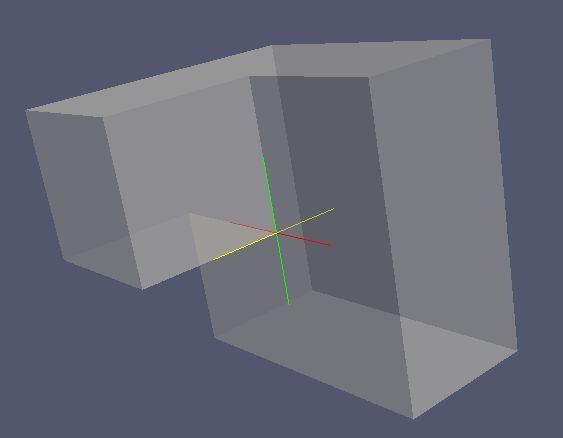
\includegraphics[width=0.45\linewidth]{images/sampleBlock1.png} \hfill
   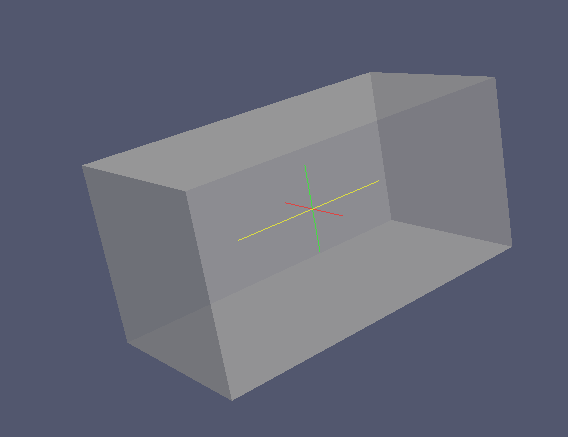
\includegraphics[width=0.45\linewidth]{images/sampleBlock2.png}
   \caption{Sample models of 2x2x2 blocks}
   \label{fig:sampleBlocks}
\end{figure}

After model computation, next step is getting vertices and faces from model cells writing results to file. However, as we have already said, we are only interested in boundaries of the final model while now we have only boundaries of a single block. Consequently, we have to separate boundaries from the inner faces of the block on different files (boundaries separation will be explained in section~\ref{sec:LARUtils}). As we can see later, we will merge boundaries together deleting common faces on both block borders, obtaining a model without internal faces. These are pieces of code for getting the inner block model with the boundaries and for file writing:

@D get inner model and boundaries
@{models = LARUtils.computeModelAndBoundaries(imageDx, imageDy, imageDz,
					    xStart, yStart, zStart, objectBoundaryChain)

V, FV = models[1][1] # inside model
V_left, FV_left = models[2][1]
V_right, FV_right = models[3][1] # right boundary
V_top, FV_top = models[4][1] # top boundary
V_bottom, FV_bottom = models[5][1] # bottom boundary
V_front, FV_front = models[6][1] # front boundary
V_back, FV_back = models[7][1] # back boundary
@}

@D write block models to file
@{# Writing all models on disk
model_outputFilename = string(outputDirectory, "MODELS/model_output_", xBlock,
				"-", yBlock, "_", startImage, "_", endImage)
Model2Obj.writeToObj(V, FV, model_outputFilename)

left_outputFilename = string(outputDirectory, "MODELS/left_output_", xBlock,
				"-", yBlock, "_", startImage, "_", endImage)
Model2Obj.writeToObj(V_left, FV_left, left_outputFilename)

right_outputFilename = string(outputDirectory, "MODELS/right_output_", xBlock,
				"-", yBlock, "_", startImage, "_", endImage)
Model2Obj.writeToObj(V_right, FV_right, right_outputFilename)

top_outputFilename = string(outputDirectory, "MODELS/top_output_", xBlock,
				"-", yBlock, "_", startImage, "_", endImage)
Model2Obj.writeToObj(V_top, FV_top, top_outputFilename)

bottom_outputFilename = string(outputDirectory, "MODELS/bottom_output_", xBlock,
				"-", yBlock, "_", startImage, "_", endImage)
Model2Obj.writeToObj(V_bottom, FV_bottom, bottom_outputFilename)

front_outputFilename = string(outputDirectory, "MODELS/front_output_", xBlock,
				"-", yBlock, "_", startImage, "_", endImage)
Model2Obj.writeToObj(V_front, FV_front, front_outputFilename)

back_outputFilename = string(outputDirectory, "MODELS/back_output_", xBlock,
				"-", yBlock, "_", startImage, "_", endImage)
Model2Obj.writeToObj(V_back, FV_back, back_outputFilename) @}

This is the \texttt{processFunction} for this pipeline step

@D image conversion process
@{function imageConversionProcess(sliceDirectory,
			      startImage, endImage,
			      imageDx, imageDy,
			      imageWidth, imageHeight,
			      outputDirectory,
			      centroids, boundaryMat)
  """
  Support function for converting a stack of image on a single
  independent process
  """

  @< image read and centroids sort @>
  
  @< block iteration @>

      @< get image slice @>
      
      if(length(chains3D) != 0)
        # Computing boundary chain
        debug("chains3d = ", chains3D)
        debug("Computing boundary chain")
        objectBoundaryChain = Lar2Julia.larBoundaryChain(boundaryMat, chains3D)
        debug("Converting models into obj")
        try
          mkdir(string(outputDirectory, "MODELS"))
        catch
        end
        @< get inner model and boundaries @>
        
        @< write block models to file @>
      else
        debug("Model is empty")
      end
    end
  end
end @}

This is the code for starting this pipeline step:

@D pixels to voxels conversion step
@{@@time iterateOnBlocks(sliceDirectory,
                  imageHeight, imageWidth, imageDepth,
                  imageDx, imageDy, imageDz,
                  imageConversionProcess, outputDirectory,
                  centroidsCalc, boundaryMat) @}
                  
\subsubsection{Boundaries merge step}\label{sec:boundariesStep}
Next step of our pipeline consists in \textit{boundaries merge}. In fact, we have already seen that for every non-empty cell we create files for the inner parts and for the boundaries of the block. So if we want a final model without boundaries between internal blocks, we need to merge them removing duplicated faces on both sides (see Section~\ref{sec:removeDoubleFacesAndVerticesFromBoundaries} for a better explanation of this step). The following is the \texttt{processFunction}:

@D boundary merge process function
@{function mergeBoundariesProcess(modelDirectory,
				  startImage, endImage,
				  imageDx, imageDy,
				  imageWidth, imageHeight,
				  outputDirectory = None,
				  centroidsCalc = None, boundaryMat = None)
  """
  Helper function for mergeBoundaries.
  It is executed on different processes

  modelDirectory: Directory containing model files
  startImage: Block start image
  endImage: Block end image
  imageDx, imageDy: x and y sizes of the grid
  imageWidth, imageHeight: Width and Height of the image
  """
  for xBlock in 0:(imageWidth / imageDx - 1)
    for yBlock in 0:(imageHeight / imageDy - 1)

      # Merging right Boundary
      firstPath = string(modelDirectory, "/right_output_", xBlock, "-", yBlock,
			"_", startImage, "_", endImage)
      secondPath = string(modelDirectory, "/left_output_", xBlock, "-", yBlock + 1,
			"_", startImage, "_", endImage)
      mergeBoundariesAndRemoveDuplicates(firstPath, secondPath)

      # Merging top boundary
      firstPath = string(modelDirectory, "/top_output_", xBlock, "-", yBlock,
			 "_", startImage, "_", endImage)
      secondPath = string(modelDirectory, "/bottom_output_", xBlock, "-", yBlock,
			 "_", endImage, "_", endImage + (endImage - startImage))
      mergeBoundariesAndRemoveDuplicates(firstPath, secondPath)

      # Merging front boundary
      firstPath = string(modelDirectory, "/front_output_", xBlock, "-", yBlock,
			"_", startImage, "_", endImage)
      secondPath = string(modelDirectory, "/back_output_", xBlock + 1, "-", yBlock,
			"_", startImage, "_", endImage)
      mergeBoundariesAndRemoveDuplicates(firstPath, secondPath)
    end
  end
end @}

For every block we do the following merges:
\begin{itemize}
 \item right boundary with the left boundary of the next block on the right
 \item top boundary with the bottom boundary of the next block on the top
 \item front boundary with the back boundary of the next block on the front
\end{itemize}

\begin{figure}[htb] %  figure placement: here, top, bottom
   \centering
   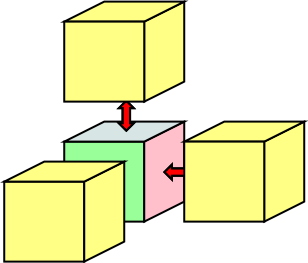
\includegraphics[width=0.30\linewidth]{images/BoundaryMergeIteration.png}
   \caption{Merging of boundary faces. For a single block we need adjacent blocks on the right, top and front}
   \label{fig:boundaryMergeIteration}
\end{figure}

all merges are executed by the function \texttt{mergeBoundariesAndRemoveDuplicates} which does the work calling the \texttt{Model2Obj} and \texttt{LARUtils} libraries for loading and cleaning of the boundaries models.

@D merge boundaries utility function
@{function mergeBoundariesAndRemoveDuplicates(firstPath, secondPath)
  """
  Merge two boundary files removing common faces between
  them

  firstPath, secondPath: Prefix of paths to merge
  """

  firstPathV = string(firstPath, "_vtx.stl")
  firstPathFV = string(firstPath, "_faces.stl")

  secondPathV = string(secondPath, "_vtx.stl")
  secondPathFV = string(secondPath, "_faces.stl")

  if(isfile(firstPathV) && isfile(secondPathV))

    V, FV = Model2Obj.getModelsFromFiles([firstPathV, secondPathV],
					 [firstPathFV, secondPathFV])
    V, FV = LARUtils.removeVerticesAndFacesFromBoundaries(V, FV)

    # Writing model to file
    rm(firstPathV)
    rm(firstPathFV)
    rm(secondPathV)
    rm(secondPathFV)
    Model2Obj.writeToObj(V, FV, firstPath)
  end
end @}

This is the code used to start this pipeline step:

@D boundaries merge step
@{@@time iterateOnBlocks(string(outputDirectory, "MODELS"),
                  imageHeight, imageWidth, imageDepth,
                  imageDx, imageDy, imageDz,
                  mergeBoundariesProcess, None,
                  None, None) @}
                
\subsubsection{Block merge step}\label{sec:blockMergeStep}

At this step of the computation, we have files with the inner parts of a single block model and the remaining boundaries. Now we need to merge the blocks removing double vertices and faces, so we can save space and prepare our model to the \textit{smoothing step}. This is the code of the \texttt{processFunction}:

@D Block merge process function
@{function mergeBlocksProcess(modelDirectory,
			      startImage, endImage,
			      imageDx, imageDy,
			      imageWidth, imageHeight,
			      outputDirectory = None,
			      centroidsCalc = None, boundaryMat = None)
  """
  Helper function for mergeBlocks.
  It is executed on different processes

  modelDirectory: Directory containing model files
  startImage: Block start image
  endImage: Block end image
  imageDx, imageDy: x and y sizes of the grid
  imageWidth, imageHeight: Width and Height of the image
  """
  for xBlock in 0:(imageWidth / imageDx - 1)
    for yBlock in 0:(imageHeight / imageDy - 1)

      blockCoordsV = string(xBlock, "-", yBlock, "_", startImage,
			    "_", endImage, "_vtx.stl")
      blockCoordsFV = string(xBlock, "-", yBlock, "_", startImage,
			    "_", endImage, "_faces.stl")

      arrayV = [string(modelDirectory, "/left_output_", blockCoordsV),
                string(modelDirectory, "/right_output_", blockCoordsV),
                string(modelDirectory, "/top_output_", blockCoordsV),
                string(modelDirectory, "/bottom_output_", blockCoordsV),
                string(modelDirectory, "/front_output_", blockCoordsV),
                string(modelDirectory, "/back_output_", blockCoordsV),
                string(modelDirectory, "/model_output_", blockCoordsV)]

      arrayFV = [string(modelDirectory, "/left_output_", blockCoordsFV),
                 string(modelDirectory, "/right_output_", blockCoordsFV),
                 string(modelDirectory, "/top_output_", blockCoordsFV),
                 string(modelDirectory, "/bottom_output_", blockCoordsFV),
                 string(modelDirectory, "/front_output_", blockCoordsFV),
                 string(modelDirectory, "/back_output_", blockCoordsFV),
                 string(modelDirectory, "/model_output_", blockCoordsFV)]

      V, FV = Model2Obj.getModelsFromFiles(arrayV, arrayFV)
      V, FV = LARUtils.removeDoubleVerticesAndFaces(V, FV, 0)
      for i in 1:length(arrayV)
        if(isfile(arrayV[i]))
          rm(arrayV[i])
          rm(arrayFV[i])
        end
      end

      Model2Obj.writeToObj(V, FV, string(modelDirectory, "/model_output_",
                               xBlock, "-", yBlock, "_", startImage, "_", endImage))
    end
  end
end @}

For a better explanation of the \texttt{LARUtils} function that remove duplicated vertices, you can see Section~\ref{sec:doubleverticesandfacesremoval}

This is the code for block merge starting
@D block merge step
@{@@time iterateOnBlocks(string(outputDirectory, "MODELS"),
                  imageHeight, imageWidth, imageDepth,
                  imageDx, imageDy, imageDz,
                  mergeBlocksProcess, None,
                  None, None) @}


\subsubsection{Smoothing step}\label{sec:smoothingStep}

Now we have obtained models without internal boundaries between blocks and without double vertices and faces in a single block. However this partial model has squared edges, so we need to smooth them. The \texttt{processFunction} for this step, is the following:

@D Smooth block process function
@{function smoothBlocksProcess(modelDirectory,
			      startImage, endImage,
			      imageDx, imageDy,
			      imageWidth, imageHeight,
			      outputDirectory = None,
			      centroidsCalc = None, boundaryMat = None)
  """
  Smoothes a block in a single process

  modelDirectory: Path of the directory containing all blocks
                  that will be smoothed
  startImage, endImage: start and end image for this block
  imageDx, imageDy: sizes of the grid
  imageWidth, imageHeight: sizes of the images
  """

  for xBlock in 0:(imageWidth / imageDx - 1)
    for yBlock in 0:(imageHeight / imageDy - 1)

      # Loading the current block model
      blockFileV = string(modelDirectory, "/model_output_", xBlock, "-", yBlock,
			  "_", startImage, "_", endImage, "_vtx.stl")
      blockFileFV = string(modelDirectory, "/model_output_", xBlock, "-", yBlock,
			  "_", startImage, "_", endImage, "_faces.stl")

      if isfile(blockFileV)
        # Loading only model of the current block
        blockModelV, blockModelFV = Model2Obj.getModelsFromFiles([blockFileV], [blockFileFV])
        blockModelV, blockModelFV = LARUtils.removeDoubleVerticesAndFaces(blockModelV, blockModelFV, 0)

        # Loading a unique model from this block and its adjacents
        modelsFiles = Array(String, 0)
        for x in xBlock - 1:xBlock + 1
          for y in yBlock - 1:yBlock + 1
            for z in range(startImage - (endImage - startImage),(endImage - startImage), 3)
              push!(modelsFiles, string(modelDirectory, "/model_output_",
					x, "-", y, "_", z, "_", z + (endImage - startImage)))
            end
          end
        end

        modelsFilesV = map((s) -> string(s, "_vtx.stl"), modelsFiles)
        modelsFilesFV = map((s) -> string(s, "_faces.stl"), modelsFiles)

        modelV, modelFV = Model2Obj.getModelsFromFiles(modelsFilesV, modelsFilesFV)
        modelV, modelFV = LARUtils.removeDoubleVerticesAndFaces(modelV, modelFV, 0)

        # Now I have to save indices of vertices of the current block model
        blockVerticesIndices = Array(Int, 0)
        for i in 1:length(blockModelV)
          for j in 1:length(modelV)
            if blockModelV[i] == modelV[j]
              push!(blockVerticesIndices, j)
            end
          end

          # Now I can apply smoothing on this model
          V_sm, FV_sm = Smoother.smoothModel(modelV, modelFV)

          # Now I have to get only block vertices and save them on the new model
          V_final = Array(Array{Float64}, 0)
          for i in blockVerticesIndices
            push!(V_final, V_sm[i])
          end
          outputFilename = string(modelDirectory, "/smoothed_output_", xBlock, "-",
				  yBlock, "_", startImage, "_", endImage)
          Model2Obj.writeToObj(V_final, blockModelFV, outputFilename)
        end
      end
    end
  end
end @}

An explanation of the smoothing algorithm used there, can be found in Section~\ref{sec:smoothing}. What we need to remember here, is the importance of having the adjacent vertices for every vertex of our block. In fact, according to the chosen smoothing algorithm, every vertex is replaced with a new one with coordinates computed from the mean positions of its adjacent. However, loading of the entire model into memory cannot be done because of its sizes; so we created a simple algorithm which loads only near blocks to the current one.
In fact, for every block we want to smooth, we load the twenty six adjacent blocks on all directions and the chosen one. We create a unique model with it (removing double vertices and faces) and then smoothing it with the algorithm in \texttt{Smoother} module. Finally we save only smoothed vertices for the chosen block and continue with the other blocks. In Figure~\ref{fig:SmoothingBlocks} there is a graphical explanation for the algorithm.

\begin{figure}[htb] %  figure placement: here, top, bottom
   \centering
   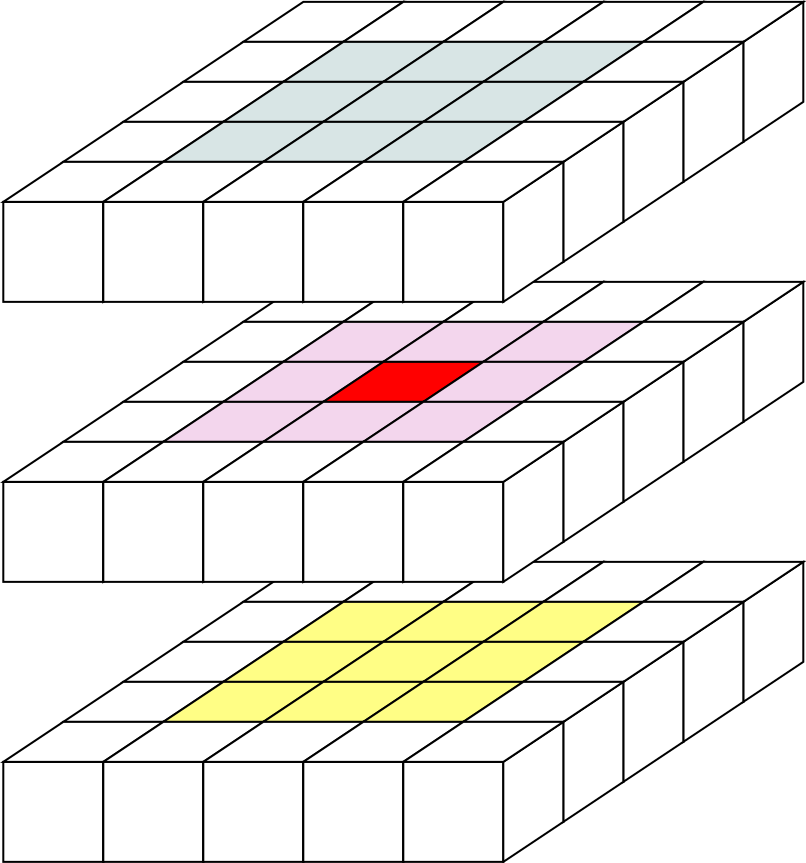
\includegraphics[width=0.30\linewidth]{images/SmoothingBlocks.png}
   \caption{Smoothing of a single block. The red block at the center of the figure is the current one, while the other twenty six colored ones are the blocks that will be part of the model which will be smoothed for this iteration}
   \label{fig:SmoothingBlocks}
\end{figure}

Moreover, this \texttt{processFunction} can only execute a single iteration of the smoothing algorithm, so we need a function that can be able to execute more times the algorithm:

@D execute smoothing function
@{function smoothBlocks(modelDirectory,
                      imageHeight, imageWidth, imageDepth,
                      imageDx, imageDy, imageDz)
  """
  Smoothes all blocks of the
  model
  """
   
  iterations = 1
  for i in 1:iterations
    info("Iteration ", i)

    iterateOnBlocks(modelDirectory,
                    imageHeight, imageWidth, imageDepth,
                    imageDx, imageDy, imageDz,
                    smoothBlocksProcess,
                    None, None, None)

    # Moving smoothed file for next iterations

    beginImageStack = 0
    endImage = beginImageStack
    for zBlock in 0:(imageDepth / imageDz - 1)
      startImage = endImage
      endImage = startImage + imageDz
      for xBlock in 0:(imageWidth / imageDx - 1)
        for yBlock in 0:(imageHeight / imageDy - 1)

          f_V = string(modelDirectory, "/smoothed_output_", xBlock, "-", yBlock, "_",
                       startImage, "_", endImage, "_vtx.stl")
          f_FV = string(modelDirectory, "/smoothed_output_", xBlock, "-", yBlock, "_",
                        startImage, "_", endImage, "_faces.stl")

          if(isfile(f_V))
            if VERSION >= v"0.4"
              mv(f_V, replace(f_V, "smoothed", "model"), remove_destination = true)
              mv(f_FV, replace(f_FV, "smoothed", "model"), remove_destination = true)
            else
              mv(f_V, replace(f_V, "smoothed", "model"))
              mv(f_FV, replace(f_FV, "smoothed", "model"))
            end
          end
        end
      end
    end
  end
end @}

We can see that after every smoothing iteration on the complete model, we need to rename the output files for the next iterations. In fact, this parallel algorithm works because for every block we do not need the current smoothed vertices for the adjacent blocks but only the old ones. However after first iteration we will have a lot of files with both the new smoothed model and the previous version; as a consequence we need to remove the old model and prepare the smoothed data for the next smoothing iteration.
This is the code for starting this step:

@D smoothing step
@{@@time smoothBlocks(string(outputDirectory, "MODELS"),
	      imageHeight, imageWidth, imageDepth,
	      imageDx, imageDy, imageDz) @}
                      
\subsubsection{Model creation step}\label{sec:mergeStep}

At this point of the pipeline, we have a lot of files containing models for a single block; now we can merge them in a unique obj file. As we will see in Section~\ref{sec:Model2Obj}, there are two different algorithms for file merging. The first one use a serial merging and it is better for traditional filesystems. The other one use a parallel algorithm which 
is better on a distributed filesystem. This is the code for invocation of the step:

@D final file merge
@{if parallelMerge
  @@time Model2Obj.mergeObjParallel(string(outputDirectory, "MODELS"))
else
  @@time Model2Obj.mergeObj(string(outputDirectory, "MODELS")) @}

%===============================================================================
\section{GenerateBorderMatrix}\label{sec:GenerateBorderMatrix}
%===============================================================================
This module has the responsibility for the generation of the border matrix operator for models boundary computation.

\subsection{Module imports}\label{sec:importsBorderMatrix}

These are modules needed for this part of the package and the public functions exported

@D modules import GenerateBorderMatrix
@{import LARUtils
using PyCall

import JSON

export computeOriented3Border, writeBorder, getOriented3BorderPath

@@pyimport sys
# Search for python modules in package folder
unshift!(PyVector(pyimport("sys")["path"]), Pkg.dir("ImagesToLARModel/src"))
@@pyimport larcc # Importing larcc from local folder
@}

We can notice some lines for importing \texttt{larcc} python library, which will be used in subsection~\ref{sec:transformBorder}

\subsection{Get border matrix from file}\label{sec:getBorderMatrix}

As we have already seen in previous sections, we need to compute boundaries for every block of the model grid. This can be done using the topological boundary operator from LAR package. However, the resulting matrix depends only on grid sizes; so it could be reused for other models. Consequently first time we need a border operator we compute it and then save it on disk for next conversions. This function does that work searching for a file containing the border and, if it does not exist, calculate and save it: 

@D get Border matrix
@{function getOriented3BorderPath(borderPath, nx, ny, nz)
  """
  Try reading 3-border matrix from file. If it fails matrix
  is computed and saved on disk in JSON format

  borderPath: path of border directory
  nx, ny, nz: image dimensions
  """

  filename = string(borderPath,"/border_", nx, "-", ny, "-", nz, ".json")
  if !isfile(filename)
    border = computeOriented3Border(nx, ny, nz)
    writeBorder(border, filename)
  end
  return filename

end @}

\subsection{Write border matrix on file}\label{sec:writeBorderMatrix}

We have already seen that for performance reasons border operator matrix is saved on file; here we will see code used for this scope. Firstly, we have defined a function \texttt{writeBorder}, which takes as parameters a \texttt{PyObject} containing a matrix (computed in subsection~\ref{sec:computeBorder}) and the output file path. When porting of \texttt{larcc} library will be completed, code for conversion of python csr matrix into csc julia matrix will not be necessary.

@D write Border matrix
@{function writeBorder(boundaryMatrix, outputFile)
  """
  Write 3-border matrix on json file

  boundaryMatrix: matrix to write on file
  outputFile: path of the outputFile
  """

  fullBorder = pycall(boundaryMatrix["toarray"], PyAny)
  cscBorder = sparse(fullBorder)
  row = findn(cscBorder)[1]
  col = findn(cscBorder)[2]
  data = nonzeros(cscBorder)

  matrixObj = MatrixObject(0, 0, row, col, data)

  outfile = open(string(outputFile), "w")
  JSON.print(outfile, matrixObj)
  close(outfile)
end @}

We can see that, in final JSON file, we write an object called \texttt{MatrixObject} which has the following definition:

@D Matrix object for JSON file
@{type MatrixObject
  ROWCOUNT
  COLCOUNT
  ROW
  COL
  DATA
end @}

The most important fields of this object are the last three ones; the first two contain all coordinates of the non-zero elements, the last contains all non-zero elements of the sparse matrix. So considering the full matrix \textit{V} we will have that $S[ROW[k], COL[k]] = V[k]$.

\subsection{Compute border matrix}\label{sec:computeBorder}

Here we can see code used for computation of the border operator. As we can see, we call the python \texttt{larcc} module, from the LAR module, which returns a \texttt{PyObject} containing a \textit{sparse csr matrix}. In next versions this function will be probably changed and the code for boundary computation will be moved in \texttt{LAR2Julia} module (also transforming all csr matrix in csc matrix) avoiding python calls.

@D compute border matrix
@{# Compute the 3-border operator
function computeOriented3Border(nx, ny, nz)
  """
  Compute the 3-border matrix using a modified
  version of larcc
  """
  V, bases = LARUtils.getBases(nx, ny, nz)
  boundaryMat = larcc.signedCellularBoundary(V, bases)
  return boundaryMat

end @}

\subsection{Transform border matrix}\label{sec:transformBorder}

Last function we will see, extracts the \texttt{MatrixObject} in Section~\ref{sec:writeBorderMatrix} converting it into a common Julia csc sparse matrix

@D transform border matrix in csc format
@{function getBorderMatrix(borderFilename)
  """
  Get the border matrix from json file and convert it in
  CSC format
  """
  # Loading borderMatrix from json file
  borderData = JSON.parsefile(borderFilename)
  
  # Converting Any arrays into Int arrays
  row = Array(Int64, length(borderData["ROW"]))
  col = Array(Int64, length(borderData["COL"]))
  data = Array(Int64, length(borderData["DATA"]))

  for i in 1: length(borderData["ROW"])
    row[i] = borderData["ROW"][i]
  end

  for i in 1: length(borderData["COL"])
    col[i] = borderData["COL"][i]
  end

  for i in 1: length(borderData["DATA"])
    data[i] = borderData["DATA"][i]
  end
  return sparse(row, col, data)
end @}

%===============================================================================
\section{Lar2Julia}\label{sec:Lar2Julia}
%===============================================================================
This module contains functions used in LAR library which are converted using Julia syntax. Next versions of the software will contain more and more functions from the original LAR library (which is written in python)

\subsection{Module imports}\label{sec:Lar2JuliaImports}

These are modules used for \texttt{Lar2Julia} and the public functions

@D modules import Lar2Julia
@{import JSON

using Logging

export larBoundaryChain, cscChainToCellList @}

\subsection{Get boundary chain from a model}\label{sec:boundaryChain}

Now we will observe how to compute the boundary chain of a LAR model given the list of non-empty cells and the boundary operator stored as a csc sparse matrix.
This algorithm is very simply: firstly we need to convert the list of cells into a sparse array containing the LAR model.
So, the resulting array (which will be called \texttt{cscChain}) will contain a one  for every cscChain[ i ][ 1 ] $\forall i \in$ \texttt{brcCellList}. Next, we just have to compute the product between the two sparse matrices and convert all values of the result into one of these: \{-1; +1; 0\} using function \texttt{cscBinFilter}.

@D get boundary chain
@{function larBoundaryChain(cscBoundaryMat, brcCellList)
  """
  Compute boundary chains
  """

  # Computing boundary chains
  n = size(cscBoundaryMat)[1]
  m = size(cscBoundaryMat)[2]

  debug("Boundary matrix size: ", n, "\t", m)

  data = ones(Int64, length(brcCellList))

  i = Array(Int64, length(brcCellList))
  for k in 1:length(brcCellList)
    i[k] = brcCellList[k] + 1
  end

  j = ones(Int64, length(brcCellList))

  debug("cscChain rows length: ", length(i))
  debug("cscChain columns length: ", length(j))
  debug("cscChain data length: ", length(brcCellList))

  debug("rows ", i)
  debug("columns ", j)
  debug("data ", data)

  cscChain = sparse(i, j, data, m, 1)
  cscmat = cscBoundaryMat * cscChain
  out = cscBinFilter(cscmat)
  return out
end

function cscBinFilter(CSCm)
  k = 1
  data = nonzeros(CSCm)
  sgArray = copysign(1, data)

  while k <= nnz(CSCm)
    if data[k] % 2 == 1 || data[k] % 2 == -1
      data[k] = 1 * sgArray[k]
    else
      data[k] = 0
    end
    k += 1
  end

  return CSCm
end
@}

\subsection{Get oriented cells from a chain}\label{sec:getCellsFromChain}

Another operation that could be useful (even if it is not actually used in the package) consists in getting of \textit{``+1''} oriented cells from a chain. For obtaining this result, it is necessary to get all non-zeros element from the sparse Julia array (remembering that if the user manually write a zero into the array it will be returned from \texttt{nonzeros} function anyway) and then returning only indices of cells that have a ``+1'' in nonzero element array.

@D get oriented cells from a chain
@{function cscChainToCellList(CSCm)
  """
  Get a csc containing a chain and returns
  the cell list of the "+1" oriented faces
  """
  data = nonzeros(CSCm)
  # Now I need to remove zero element (problem with Julia nonzeros)
  nonzeroData = Array(Int64, 0)
  for n in data
    if n != 0
      push!(nonzeroData, n)
    end
  end

  cellList = Array(Int64,0)
  for (k, theRow) in enumerate(findn(CSCm)[1])
    if nonzeroData[k] == 1
      push!(cellList, theRow)
    end
  end
  return cellList
end @}

\subsection{Transform relationships from arrays of arrays to a sparse matrix}\label{sec:transformSparse}

Another function which can be useful for our purposes is conversion between different representations of the LAR relationships. For example we often use a representation based on list of list of int but if we want to apply topological operators (such as the incident operators) we need to convert it into a matrix of values. In Figure~\ref{fig:LARRepresentations} we can see an example of a LAR relationship with different representations.

\begin{figure}[htb] %  figure placement: here, top, bottom
   \centering
   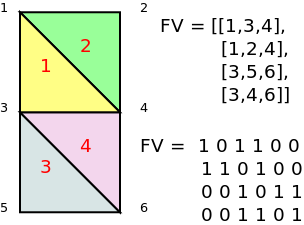
\includegraphics[width=0.45\linewidth]{images/LARRepresentations.png}
   \caption{Different representations for faces of a simple LAR model. the first one is based on a list of list of int, while the other is a simple matrix where for every value we have $FV[i][j] = 1 \iff $ \textit{face i contains the vertex j} }
   \label{fig:LARRepresentations}
\end{figure}

@D transform relationships to csc
@{function relationshipListToCSC(larRelation)
  """
  Get a LAR relationship
  and convert it into a CSC matrix
  """

  # Build I and J arrays for creation of
  # sparse matrix
  data = Array(Int, 0)
  I = Array(Int, 0)
  J = Array(Int, 0)
  for (k,row) in enumerate(larRelation)
    for col in row
      push!(I, k)
      push!(J, col)
      push!(data, 1)
    end
  end

  return sparse(I, J, data)
end @}

%===============================================================================
\section{LARUtils}\label{sec:LARUtils}
%===============================================================================

This module contains functions used for manipulation of LAR models

\subsection{Module imports}\label{sec:LARUtilsImports}

These are modules used in \texttt{LARUtils} and the functions exported

@D modules import LARUtils
@{using Logging

export ind, invertIndex, getBases, removeDoubleVerticesAndFaces,
    computeModel, computeModelAndBoundaries
@}

\subsection{Transformation from matrix to array}\label{sec:matrixTransform}

First utility functions we will see, transform a matrix into an array and vice versa. We have already seen in section~\ref{sec:conversionProcess} uses of this linearized matrices; now we can focus on code for transformation.

@D conversion from matrix to array
@{function ind(x, y, z, nx, ny)
    """
    Transform coordinates into linearized matrix indexes
    """
    return x + (nx + 1) * (y + (ny + 1) * (z))
end @}

Here we have defined also the inverse transformation from the array to the matrix, which is useful for obtaining vertices coordinates from a cell

@D conversion from array to matrix
@{function invertIndex(nx,ny,nz)
  """
  Invert indexes
  """
  nx, ny, nz = nx + 1, ny + 1, nz + 1
  function invertIndex0(offset)
      a0, b0 = trunc(offset / nx), offset % nx
      a1, b1 = trunc(a0 / ny), a0 % ny
      a2, b2 = trunc(a1 / nz), a1 % nz
      return b0, b1, b2
  end
  return invertIndex0
end @}

\subsection{Get bases of a LAR model}\label{sec:getBases}

For generation of LAR models from an array of non-empty cells, we need to define a function for obtaining a base for every model, which will contain all LAR relationships:
\begin{itemize}
 \item \textbf{V}: the array of vertices of a LAR model
 \item \textbf{VV}: the relationship between a vertex and itself
 \item \textbf{EV}: the relationship between an edge and its vertices
 \item \textbf{FV}: the relationship between a face and its vertices
 \item \textbf{CV}: the relationship between a cell and its vertices
\end{itemize}

From a geometrical point of view these bases create a chain composed from $nx \times ny \times nz$ square cells (where nx ny and nz are the grid size).

\begin{figure}[htb] %  figure placement: here, top, bottom
   \centering
   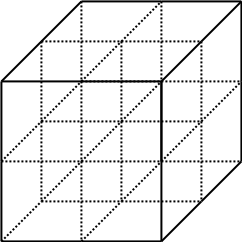
\includegraphics[width=0.25\linewidth]{images/larbasis.png}
   \caption{LAR bases geometry for a $2 \times 2 \times 2$ grid}
   \label{fig:larbasis}
\end{figure}

Now we will see in details how to obtain all LAR relationships.\\
First of all we need to compute vertices for the geometry:

@D compute vertices
@{# Calculating vertex coordinates (nx * ny * nz)
V = Array{Int64}[]
for z in 0:nz
  for y in 0:ny
    for x in 0:nx
      push!(V,[x,y,z])
    end
  end
end @}

So we assume that our cube geometry has only integers coordinates that can vary from (0,0,0) to (nx,ny,nz)

Next we have to compute the CV relationship:

@D compute CV
@{# Building CV relationship
CV = Array{Int64}[]
for z in 0:nz-1
  for y in 0:ny-1
    for x in 0:nx-1
      push!(CV,the3Dcell([x,y,z]))
    end
  end
end @}

For every coordinate in the space delimited by the grid size, it is called function \texttt{the3Dcell}, which get the coordinate values returning a cell in the three-dimensional space:

@D compute three-dimensional cells
@{function the3Dcell(coords)
  x,y,z = coords
  return [ind(x,y,z,nx,ny), ind(x+1,y,z,nx,ny), ind(x,y+1,z,nx,ny),
	  ind(x,y,z+1,nx,ny), ind(x+1,y+1,z,nx,ny), ind(x+1,y,z+1,nx,ny),
	  ind(x,y+1,z+1,nx,ny), ind(x+1,y+1,z+1,nx,ny)]
end
@}

Now we have to compute the FV relationship, which will be widely used in this package:

@D compute FV
@{# Building FV relationship
FV = Array{Int64}[]
v2coords = invertIndex(nx,ny,nz)

for h in 0:(length(V)-1)
  x,y,z = v2coords(h)

  if (x < nx) && (y < ny)
    push!(FV, [h,ind(x+1,y,z,nx,ny),ind(x,y+1,z,nx,ny),ind(x+1,y+1,z,nx,ny)])
  end

  if (x < nx) && (z < nz)
    push!(FV, [h,ind(x+1,y,z,nx,ny),ind(x,y,z+1,nx,ny),ind(x+1,y,z+1,nx,ny)])
  end

  if (y < ny) && (z < nz)
    push!(FV,[h,ind(x,y+1,z,nx,ny),ind(x,y,z+1,nx,ny),ind(x,y+1,z+1,nx,ny)])
  end

end @}

Finally we have the VV relationship (which is trivial)

@D compute VV
@{# Building VV relationship
VV = map((x)->[x], 0:length(V)-1) @}

and the EV relationship

@D compute EV
@{# Building EV relationship
EV = Array{Int64}[]
for h in 0:length(V)-1
  x,y,z = v2coords(h)
  if (x < nx)
    push!(EV, [h,ind(x+1,y,z,nx,ny)])
  end
  if (y < ny)
    push!(EV, [h,ind(x,y+1,z,nx,ny)])
  end
  if (z < nz)
    push!(EV, [h,ind(x,y,z+1,nx,ny)])
  end
end @}

This is the complete code for the function \texttt{getBases}
@D get LAR bases
@{function getBases(nx, ny, nz)
  """
  Compute all LAR relations
  """

  @< compute three-dimensional cells @>

  @< compute vertices @>

  @< compute CV @>

  @< compute FV @>
  
  @< compute VV @>
  
  @< compute EV @>

  # return all basis
  return V, (VV, EV, FV, CV)
end @}

\subsection{Double vertices and faces removal}\label{sec:doubleverticesandfacesremoval}

Another useful function for our models is \textit{removal of double vertices and faces}. In fact, when we produce a LAR model getting only full cell from the geometry in Figure~\ref{fig:larbasis} we could obtain double vertices (and consequently double faces). Figure~\ref{fig:duplicates} shows an example of a model with these vertices:

\begin{figure}[htb] %  figure placement: here, top, bottom
   \centering
   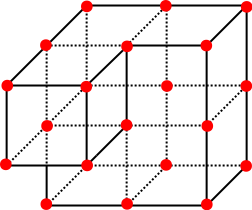
\includegraphics[width=0.25\linewidth]{images/duplicates.png}
   \caption{A sample model taken from a $2 \times 2 \times 2$ grid with double vertices between faces in red (remember that we have only the boundaries faces for the model as we have seen in section~\ref{sec:conversionProcess})}
   \label{fig:duplicates}
\end{figure}

As we can see, for every model there are a lot of double vertices, so we need to remove them for obtaining a compact representation and for next smoothing of the objects. First of all we have to identify double vertices, so it can be useful to define an order between them. Unfortunately Julia does not define a function for order array containing coordinates (which is format used in \textit{V} array); so we have to define first a custom ordering function:

@D vertices comparator function
@{function lessThanVertices(v1, v2)
  """
  Utility function for comparing vertices coordinates
  """

  if v1[1] == v2[1]
    if v1[2] == v2[2]
      return v1[3] < v2[3]
    end
    return v1[2] < v2[2]
  end
  return v1[1] < v2[1]
end @}

Now we can remove double vertices from the \textit{V} array simply ordering them and removing all consecutive equal vertices. This procedure is more complex than a simple call to Julia \texttt{unique} function for removal of double elements because we need the new vertices indices for renaming faces (as we can see later)

@D removal of double vertices
@{function removeDoubleVertices(V)
  """
  Remove double vertices from a LAR model

  V: Array containing all vertices of the model
  """

  # Sort the vertices list and returns the ordered indices
  orderedIndices = sortperm(V, lt = lessThanVertices, alg=MergeSort)

  orderedVerticesAndIndices = collect(zip(sort(V, lt = lessThanVertices),
                                          orderedIndices))
  newVertices = Array(Array{Float64}, 0)
  indices = zeros(Int, length(V))
  prevv = Void
  i = 1
  for (v, ind) in orderedVerticesAndIndices
    if v == prevv
      indices[ind] = i - 1
    else
      push!(newVertices, v)
      indices[ind] = i
      i += 1
      prevv = v
    end
  end
  return newVertices, indices
end @}

As we can see the algorithm does the following steps:
\begin{enumerate}
 \item Sort of vertices list
 \item Set the current vertex index counter to 1
 \item For every couple (\textit{vertex}, \textit{index} into V array) do:
 \begin{enumerate}
  \item If the current \textit{vertex} is equal to the previous one put into the indices array at position \textit{index} the value for the current vertex index count
  \item If the current \textit{vertex} is not equal to the previous one save it into a new V array, insert the indices array at position \textit{index} the current index count and increment it by one
 \end{enumerate}
\end{enumerate}

So at the end of this function the array \textit{newVertices} will contain all unique vertices, while the \textit{indices} array will contain the correct index for every vertex into \textit{newVertices} and the index corresponding to the saved vertex for every deleted vertex.\\

Now we can use these informations for renaming all faces.

@D renaming of faces
@{function reindexVerticesInFaces(FV, indices, offset)
  """
  Reindex vertices indices in faces array

  FV: Faces array of the LAR model
  indices: new Indices for faces
  offset: offset for faces indices
  """

  for f in FV
    for i in 1: length(f)
      f[i] = indices[f[i] - offset] + offset
    end
  end
  return FV
end @}

Here we can observe a \textit{offset} parameter, which is necessary only if we are renaming faces whose indices doesn't start from zero; actually in \texttt{ImagesToLARModel} it is always equal to zero.\\

Finally for removing double faces, we only have to call \texttt{unique} function on renamed faces. This is the final code

@D removal of double vertices and faces
@{@< vertices comparator function @>

function removeDoubleVerticesAndFaces(V, FV, facesOffset)
  """
  Removes double vertices and faces from a LAR model

  V: Array containing all vertices
  FV: Array containing all faces
  facesOffset: offset for faces indices
  """

  newV, indices = removeDoubleVertices(V)
  reindexedFaces = reindexVerticesInFaces(FV, indices, facesOffset)
  newFV = unique(FV)

  return newV, newFV

end

@< removal of double vertices @>

@< renaming of faces @> @}

\subsection{Creation of a LAR model}\label{sec:modelCreation}

Now we can see code used for creation of a LAR model given the sparse array containing full cells of our block (\textbf{objectBoundaryChain} as we had seen in Section~\ref{sec:boundaryChain}). We also need the following parameters:
\begin{itemize}
 \item \textbf{imageDx}, \textbf{imageDy}, \textbf{imageDz}: The grid size
 \item \textbf{xStart}, \textbf{yStart}, \textbf{zStart}: The coordinate offsets for the current block vertices
 \item \textbf{facesOffset}: The offset for faces of this block
\end{itemize}

First thing to do is define models that will be returned from the function:

@D models definition
@{V_model = Array(Array{Int}, 0)
FV_model = Array(Array{Int}, 0)

V_left = Array(Array{Int},0)
FV_left = Array(Array{Int},0)

V_right = Array(Array{Int},0)
FV_right = Array(Array{Int},0)

V_top = Array(Array{Int},0)
FV_top = Array(Array{Int},0)

V_bottom = Array(Array{Int},0)
FV_bottom = Array(Array{Int},0)

V_front = Array(Array{Int},0)
FV_front = Array(Array{Int},0)

V_back = Array(Array{Int},0)
FV_back = Array(Array{Int},0) @}

We can see from Figure~\ref{fig:boundaries} that our grid is divided into seven parts.

\begin{figure}[htb] %  figure placement: here, top, bottom
   \centering
   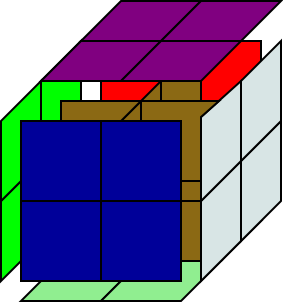
\includegraphics[width=0.25\linewidth]{images/boundaries.png}
   \caption{Decomposition of a LAR model into seven parts: the inside model (brown), the left boundary (green), the right boundary (light blue), the top boundary (purple), the bottom boundary (light green), the front boundary(blue), the back boundary (red)}
   \label{fig:boundaries}
\end{figure}

We need this decomposition because we are interested in boundaries of the entire model, while we currently have boundaries only for blocks. So we need to split the inner parts of a single block model, as we need to freely merge boundaries between adjacent blocks removing the common faces. Function for boundaries merging are shown in subsection~\ref{sec:removeDoubleFacesAndVerticesFromBoundaries}.\\

After model definition we have to get the cells indices from the block boundary chain and for every non-empty cell we have found, choose the correct model for it. We can observe that every boundary face has a fixed coordinate; for example all faces on the top boundary have the maximum z-coordinate, or faces on right boundary have the maximum y-coordinate (as shown in Figure~\ref{fig:boundariesCoordinates})

\begin{figure}[htb] %  figure placement: here, top, bottom
   \centering
   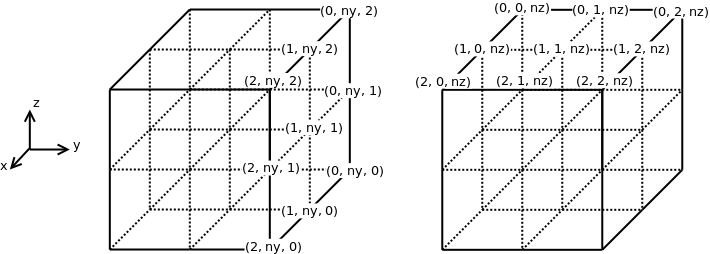
\includegraphics[width=0.90\linewidth]{images/boundariesCoordinates.png}
   \caption{Boundaries coordinates for top and right boundaries of a $2 \times 2 \times 2$ grid. We can observe that every boundary has a fixed coordinate}
   \label{fig:boundariesCoordinates}
\end{figure}

So we can define a series of functions for checking the membership of a given face to a boundary exploiting these fixed coordinates:

@D check membership of a face to a boundary
@{function isOnLeft(face, V, nx, ny, nz)
  """
  Check if face is on left boundary
  """

  for(vtx in face)
    if(V[vtx + 1][2] != 0)
      return false
    end
  end
  return true

end

function isOnRight(face, V, nx, ny, nz)
  """
  Check if face is on right boundary
  """

  for(vtx in face)
    if(V[vtx + 1][2] != ny)
      return false
    end
  end
  return true

end

function isOnTop(face, V, nx, ny, nz)
  """
  Check if face is on top boundary
  """

  for(vtx in face)
    if(V[vtx + 1][3] != nz)
      return false
    end
  end
  return true
end

function isOnBottom(face, V, nx, ny, nz)
  """
  Check if face is on bottom boundary
  """

  for(vtx in face)
    if(V[vtx + 1][3] != 0)
      return false
    end
  end
  return true
end

function isOnFront(face, V, nx, ny, nz)
  """
  Check if face is on front boundary
  """

  for(vtx in face)
    if(V[vtx + 1][1] != nx)
      return false
    end
  end
  return true
end

function isOnBack(face, V, nx, ny, nz)
  """
  Check if face is on back boundary
  """

  for(vtx in face)
    if(V[vtx + 1][1] != 0)
      return false
    end
  end
  return true
end @}

After choosing of the right model, we have to insert our face into it. We can do it with the following function, which takes vertices and faces of the base and the model, the face, and the offset of the current face for the model chosen:

@D add a face to a model
@{function addFaceToModel(V_base, FV_base, V, FV, face, vertex_count)
  """
  Insert a face into a LAR model

  V_base, FV_base: LAR model of the base
  V, FV: LAR model
  face: Face that will be added to the model
  vertex_count: Indices for faces vertices
  """
  new_vertex_count = vertex_count
  for vtx in FV_base[face]
    push!(V, [convert(Int, V_base[vtx + 1][1] + xStart),
		    convert(Int, V_base[vtx + 1][2] + yStart),
		    convert(Int, V_base[vtx + 1][3] + zStart)])
    new_vertex_count += 1
  end
  push!(FV, [vertex_count, vertex_count + 1, vertex_count + 3])
  push!(FV, [vertex_count, vertex_count + 3, vertex_count + 2])

  return new_vertex_count
end @}

As we can see, for every face we put into the model FV array two faces, in fact our final representation is not based on square faces but on triangular faces.

\begin{figure}[htb] %  figure placement: here, top, bottom
   \centering
   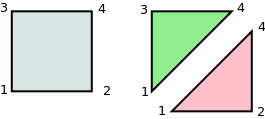
\includegraphics[width=0.40\linewidth]{images/Triangulation.png}
   \caption{Triangulation of a single face}
   \label{fig:Triangulation}
\end{figure}

This is the complete code for creation of a model

@D LAR model creation
@{@< check membership of a face to a boundary @>

function computeModelAndBoundaries(imageDx, imageDy, imageDz,
                      xStart, yStart, zStart,
                      objectBoundaryChain)
  """
  Takes the boundary chain of a part of the entire model
  and returns a LAR model splitting the boundaries

  imageDx, imageDy, imageDz: Boundary dimensions
  xStart, yStart, zStart: Offset of this part of the model
  objectBoundaryChain: Sparse csc matrix containing the cells
  """

  @< add a face to a model @>
  
  @< models definition @>

  V, bases = getBases(imageDx, imageDy, imageDz)
  FV = bases[3]

  vertex_count_model = 1
  vertex_count_left = 1
  vertex_count_right = 1
  vertex_count_top = 1
  vertex_count_bottom = 1
  vertex_count_front = 1
  vertex_count_back = 1

  # Get all cells (independently from orientation)
  b2cells = findn(objectBoundaryChain)[1]

  debug("b2cells = ", b2cells)

  for f in b2cells
    old_vertex_count_model = vertex_count_model
    old_vertex_count_left = vertex_count_left
    old_vertex_count_right = vertex_count_right
    old_vertex_count_top = vertex_count_top
    old_vertex_count_bottom = vertex_count_bottom
    old_vertex_count_front = vertex_count_front
    old_vertex_count_back = vertex_count_back

    # Choosing the right model for vertex
    if(isOnLeft(FV[f], V, imageDx, imageDy, imageDz))
      vertex_count_left = addFaceToModel(V, FV, V_left, FV_left,
				  f, old_vertex_count_left)
    elseif(isOnRight(FV[f], V, imageDx, imageDy, imageDz))
      vertex_count_right = addFaceToModel(V, FV, V_right, FV_right,
				  f, old_vertex_count_right)
    elseif(isOnTop(FV[f], V, imageDx, imageDy, imageDz))
      vertex_count_top = addFaceToModel(V, FV, V_top, FV_top,
				  f, old_vertex_count_top)
    elseif(isOnBottom(FV[f], V, imageDx, imageDy, imageDz))
      vertex_count_bottom = addFaceToModel(V, FV, V_bottom, FV_bottom,
				  f, old_vertex_count_bottom)
    elseif(isOnFront(FV[f], V, imageDx, imageDy, imageDz))
      vertex_count_front = addFaceToModel(V, FV, V_front, FV_front,
				  f, old_vertex_count_front)
    elseif(isOnBack(FV[f], V, imageDx, imageDy, imageDz))
      vertex_count_back = addFaceToModel(V, FV, V_back, FV_back,
				  f, old_vertex_count_back)
    else
      vertex_count_model = addFaceToModel(V, FV, V_model, FV_model,
				  f, old_vertex_count_model)
    end

  end

  # Removing double vertices
  return [removeDoubleVerticesAndFaces(V_model, FV_model, 0)],
  [removeDoubleVerticesAndFaces(V_left, FV_left, 0)],
  [removeDoubleVerticesAndFaces(V_right, FV_right, 0)],
  [removeDoubleVerticesAndFaces(V_top, FV_top, 0)],
  [removeDoubleVerticesAndFaces(V_bottom, FV_bottom, 0)],
  [removeDoubleVerticesAndFaces(V_front, FV_front, 0)],
  [removeDoubleVerticesAndFaces(V_back, FV_back, 0)]
end @}

\begin{figure}[htb] %  figure placement: here, top, bottom
   \centering
   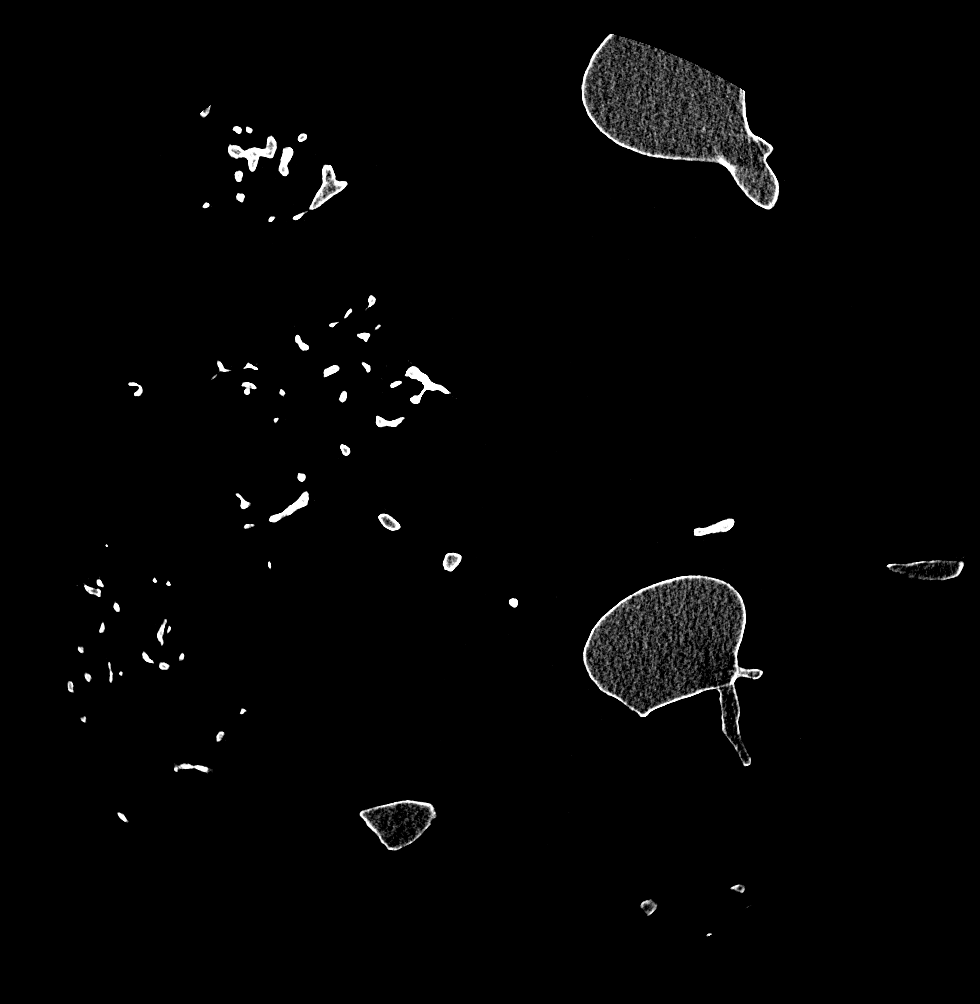
\includegraphics[width=0.30\linewidth]{images/sampleModelImage.png}
   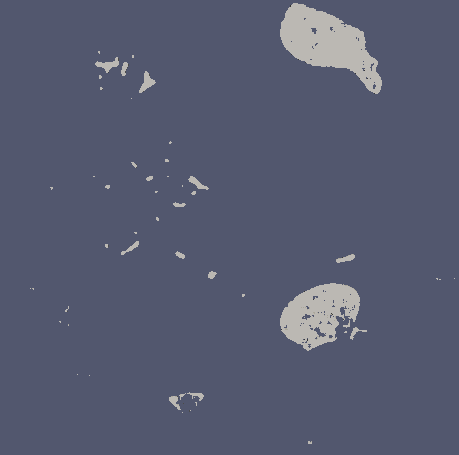
\includegraphics[width=0.30\linewidth]{images/sampleModel.png}
   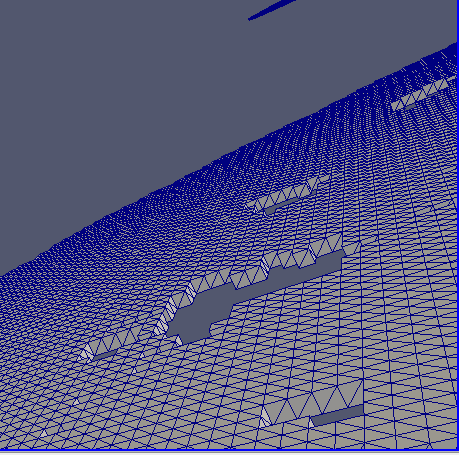
\includegraphics[width=0.30\linewidth]{images/sampleModel1.png}
   \caption{Creation of a sample model. (a) The original image (b) The three-dimensional model (c) The three-dimensional model (detail with triangular faces)}
   \label{fig:sampleModel}
\end{figure}

\subsection{Removing double faces and vertices from boundaries}\label{sec:removeDoubleFacesAndVerticesFromBoundaries}

In previous section, we have seen how to create a LAR model from the chain list. However this model contains all borders between blocks, while we are only interested in borders for the entire image. So, we will see functions for boundaries merging with removal of double faces and vertices from both sides.

\begin{figure}[htb] %  figure placement: here, top, bottom
   \centering
   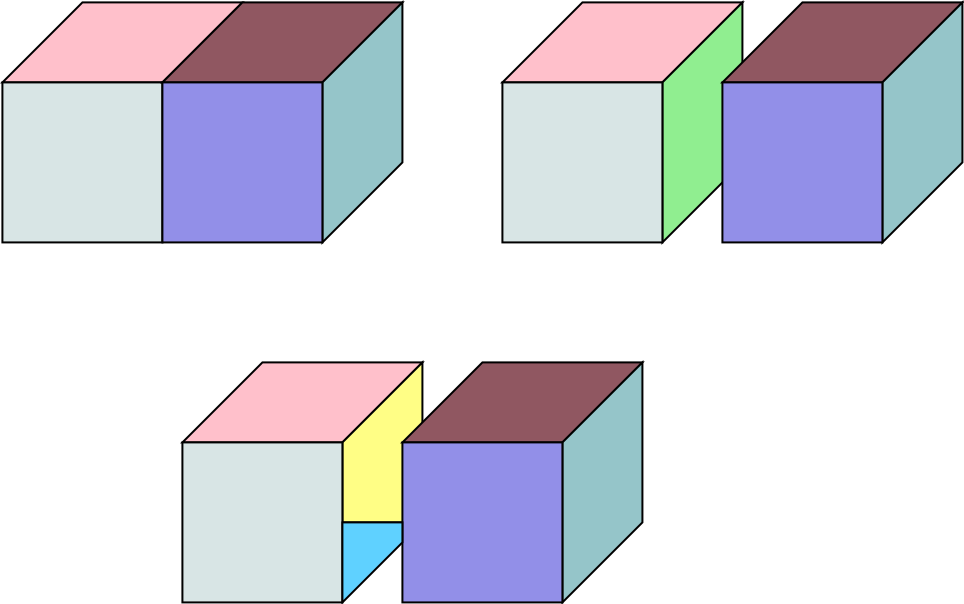
\includegraphics[width=0.40\linewidth]{images/BoundaryMerge.png}
   \caption{Removal of double faces from boundaries. (a) Two adjacent blocks (b) The same blocks exploded on x axis (c) Result of the removal on the exploded blocks}
   \label{fig:boundaryMerge}
\end{figure}

\begin{figure}[htb] %  figure placement: here, top, bottom
   \centering
   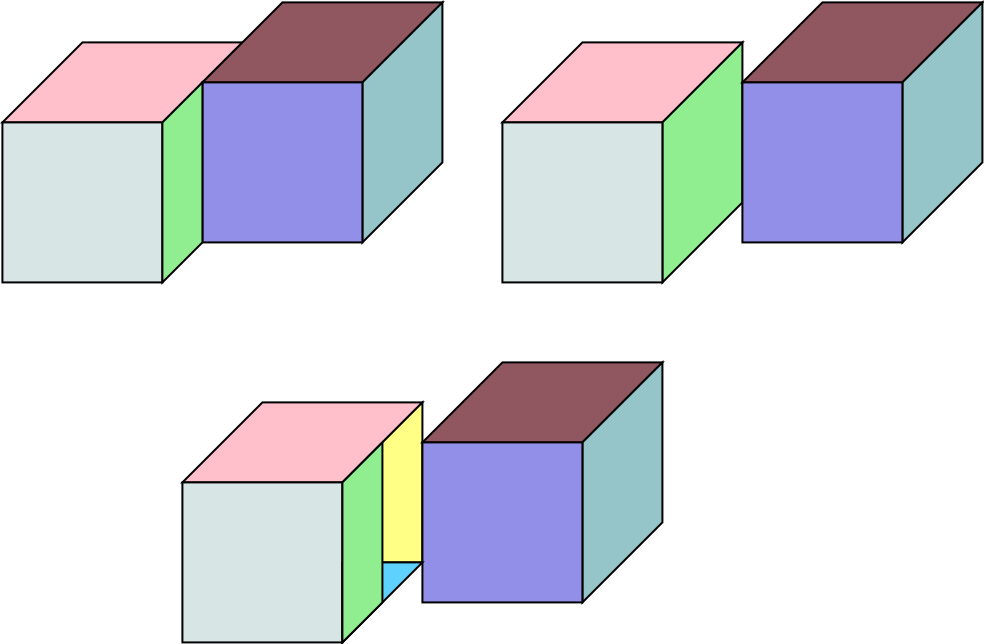
\includegraphics[width=0.40\linewidth]{images/BoundaryMerge2.png}
   \caption{Same as Figure~\ref{fig:boundaryMerge} with another model}
   \label{fig:boundaryMerge2}
\end{figure}

The algorithm for the removal is very simply. First of all we need to remove double vertices from models in the usual way using \texttt{removeDoubleVertices} function and re-indexing all faces. Next we count all elements in re-indexed faces array removing elements with more than one occurrence and create an array of faces with an explicit representation of vertices (\textit{FV\_vertices}). Now we can safely remove double vertices on the other side of the boundary without losing the correct indexing in the faces. Finally we can create the final faces array with only remaining vertices comparing coordinates in \textit{FV\_vertices} with the ones in the last vertices array.\\
Code for this function is the following:

@D Removal of double vertices and faces from boundaries
@{function removeVerticesAndFacesFromBoundaries(V, FV)
  """
  Remove vertices and faces duplicates on
  boundaries models

  V,FV: lar model of two merged boundaries
  """

  newV, indices = removeDoubleVertices(V)
  uniqueIndices = unique(indices)

  # Removing double faces on both boundaries
  FV_reindexed = reindexVerticesInFaces(FV, indices, 0)
  FV_unique = unique(FV_reindexed)

  FV_cleaned = Array(Array{Int}, 0)
  for f in FV_unique
    if(count((x) -> x == f, FV_reindexed) == 1)
      push!(FV_cleaned, f)
    end
  end

  # Creating an array of faces with explicit vertices
  FV_vertices = Array(Array{Array{Float64}}, 0)

  for i in 1 : length(FV_cleaned)
    push!(FV_vertices, Array(Array{Float64}, 0))
    for vtx in FV_cleaned[i]
      push!(FV_vertices[i], newV[vtx])
    end
  end

  V_final = Array(Array{Float64}, 0)
  FV_final = Array(Array{Int}, 0)

  # Saving only used vertices
  for face in FV_vertices
    for vtx in face
      push!(V_final, vtx)
    end
  end

  V_final = unique(V_final)

  # Renumbering FV
  for face in FV_vertices
    tmp = Array(Int, 0)
    for vtx in face
      ind = findfirst(V_final, vtx)
      push!(tmp, ind)
    end
    push!(FV_final, tmp)
  end

  return V_final, FV_final
end @}


%===============================================================================
\section{Smoother}\label{sec:Smoother}
%===============================================================================
This module contains functions used for smoothing LAR models

\subsection{Get adjacent vertices}\label{sec:adjacent}

As we will see in next subsection, for executing a smoothing algorithm we need to know adjacent vertices to a given one. So we need a \textit{VV relationship}, where for every vertex index \textit{i}, we have a list of adjacent vertices.

\begin{figure}[htb] %  figure placement: here, top, bottom
   \centering
   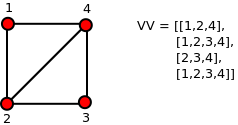
\includegraphics[width=0.40\linewidth]{images/Adjacents.png}
   \caption{\textit{VV relationship} for a simple model}
   \label{fig:adjacents}
\end{figure}

Algorithm is very simple and exploit the following property: \textit{for triangular faces all vertices are linked together}. So we just need to search for every vertex \textit{i} all faces that contain it and add all their vertices to a list. \textit{VV} will contain a concatenation of all these lists

@D get adjacent vertices
@{function adjVerts(V, FV)
  """
  Compute the adjacency graph of vertices
  of a LAR model

  V, FV: LAR model

  Returns the list of indices of vertices adjacent
  to a vertex
  """
  VV = Array{Int}[]
  for i in 1:length(V)
    row = Array(Int, 0)
    for face in FV
      if i in face
        for v in face
          push!(row, v)
        end
      end
    end
    if length(row) == 0
      push!(row, i)
    end
    push!(VV, collect(unique(row)))
  end
  return VV
end @}

\subsection{Laplacian smoothing}\label{sec:smoothing}

There are many different algorithms for mesh smoothing. The simpler and the one we used in this library is \textbf{laplacian smoothing}. For each vertex in a mesh, a new position is chosen according to local information (such as the coordinates of neighbors) and the vertex is moved there. If that mesh is topologically a rectangular grid (so each internal vertex is connected to four neighbors) then this operation produces the \textit{Laplacian} of the mesh.

\begin{figure}[htb] %  figure placement: here, top, bottom
   \centering
   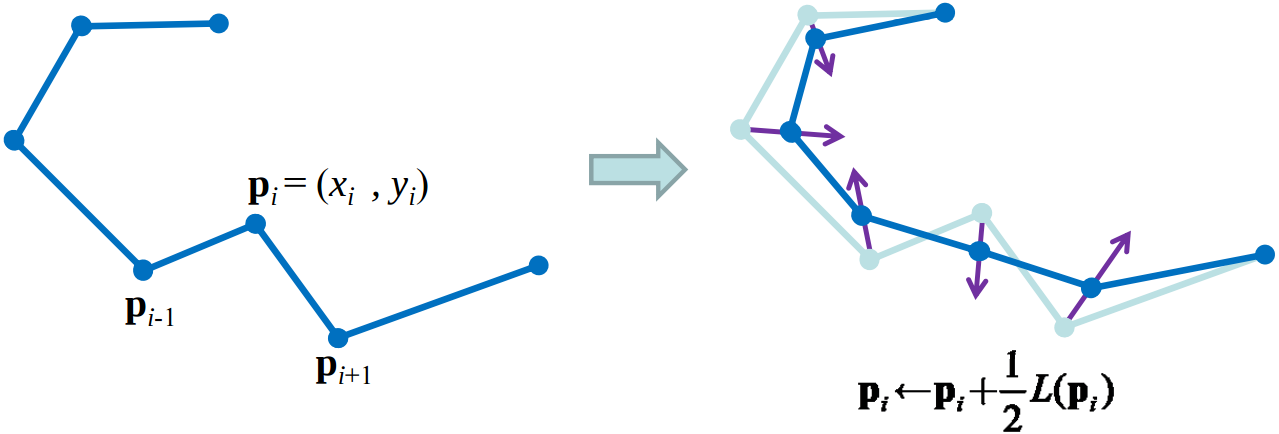
\includegraphics[width=0.60\linewidth]{images/LaplacianSmoothing.png}
   \caption{Laplacian smoothing (picture taken from the \textit{Geometry Processing Algorithms} course at Stanford University)}
   \label{fig:laplacianSmoothing}
\end{figure}

As we can see from Figure~\ref{fig:laplacianSmoothing}, with substitution of every vertex position with the mean of the neighbors positions, we can obtain a curve with smoothed edges. This procedure can be repeated many times, so we can obtain a smoother model. For example, in Figure~\ref{fig:smoothingExample}, we can see this algorithm applied on a sample mesh with three iterations.

\begin{figure}[htb] %  figure placement: here, top, bottom
   \centering
   
\includegraphics[width=0.30\linewidth]{images/SmoothingExample0.png}
   
\includegraphics[width=0.30\linewidth]{images/SmoothingExample1.png}
   \caption{Laplacian smoothing for a sample mesh. (a) Original mesh (b) Mesh after three iterations of the smoothing algorithm (picture taken from a \textit{Digital Geometry Processing} course at IMPA)}
   \label{fig:smoothingExample}
\end{figure}

This is the code for the smoothing function; it takes a single LAR model and returns the smoothed model. 

@D laplacian smoothing
@{function smoothModel(V, FV)
  """
  Execute a Laplacian smoothing on a LAR model returning
  the new smoothed model

  V, FV: LAR model
  """

  VV = adjVerts(V, FV)
  newV = Array(Array{Float64},0)
  V_temp = Array(Array{Float64},0)

  for i in 1:length(VV)
    adjs = VV[i]
    # Get all coordinates for adjacent vertices
    coords = Array(Array{Float64}, 0)
    for v in adjs
      push!(coords, V[v])
    end

    # Computing sum of all vectors
    sum = [0.0, 0.0, 0.0]
    for v in coords
      sum += v
    end

    # Computing convex combination of vertices
    push!(newV, sum/length(adjs))

  end

  return newV, FV
end @}


\begin{figure}[htb] %  figure placement: here, top, bottom
   \centering
   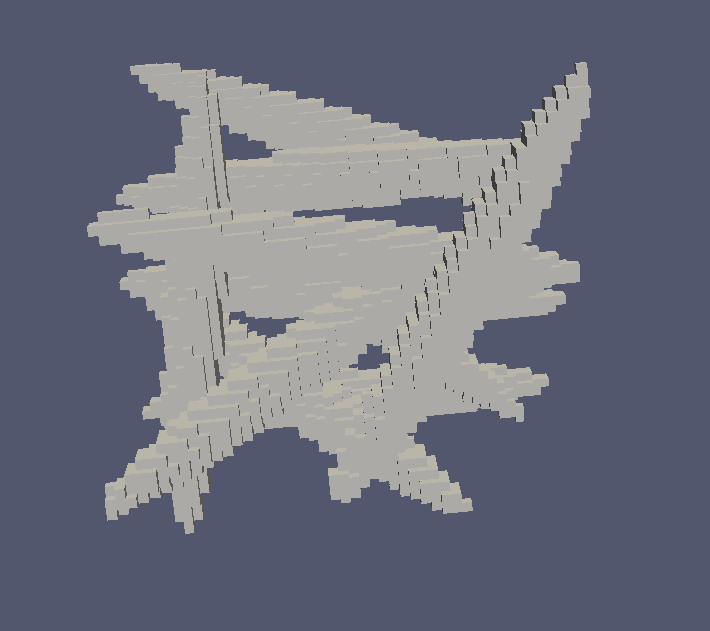
\includegraphics[width=0.40\linewidth]{images/ModelSmoothing0.png}
   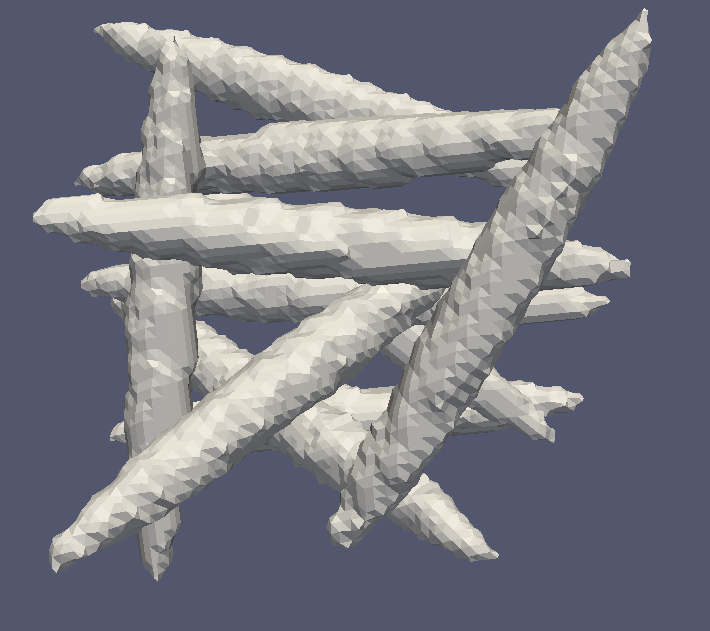
\includegraphics[width=0.40\linewidth]{images/ModelSmoothing1.png}
   \caption{Smoothing of a sample model made with ImagesToLARModel}
   \label{fig:smoothingExample}
\end{figure}

%===============================================================================
\section{Model2Obj}\label{sec:Model2Obj}
%===============================================================================

%===============================================================================
\section{Exporting the library}
%===============================================================================

\paragraph{ImagesToLARModel}
@O src/ImagesToLARModel.jl
@{module ImagesToLARModel

@< update load path @>

@< modules import ImagesToLARModel @>
@< load JSON configuration @>
@< Start conversion from JSON file @>
@< Start manual conversion @>
end
@}

\paragraph{ImagesConversion}
@O src/ImagesConversion.jl
@{module ImagesConversion

@< modules import ImagesConversion @>

@< main function for ImagesConversion @>

@< parallel block iteration @>

@< start conversion of images @>

@< image conversion process @>

@< boundary merge process function @>

@< merge boundaries utility function @>

@< Block merge process function @>

@< Smooth block process function@>

@< execute smoothing function @>

end
@}

\paragraph{GenerateBorderMatrix}

@O src/GenerateBorderMatrix.jl
@{module GenerateBorderMatrix

@< Matrix object for JSON file @>

@< modules import GenerateBorderMatrix @>

@< compute border matrix @>

@< write Border matrix  @>

@< get Border matrix @>

@< transform border matrix in csc format @>
end
@}

\paragraph{Lar2Julia}

@O src/Lar2Julia.jl
@{module Lar2Julia

@< modules import Lar2Julia @>

@< get boundary chain @>

@< get oriented cells from a chain @>

@< transform relationships to csc @>
end
@}

\paragraph{LARUtils}

@O src/LARUtils.jl
@{module LARUtils

@< modules import LARUtils @>

@< conversion from matrix to array @>

@< conversion from array to matrix @>

@< get LAR bases @>

@< removal of double vertices and faces @>

@< Removal of double vertices and faces from boundaries @>

@< LAR model creation @>
end
@}

\paragraph{Model2Obj}

@O src/Model2Obj.jl
@{module Model2Obj

import LARUtils

using Logging

export writeToObj, mergeObj, mergeObjParallel

function writeToObj(V, FV, outputFilename)
  """
  Take a LAR model and write it on obj file

  V: array containing vertices coordinates
  FV: array containing faces
  outputFilename: prefix for the output files
  """

  if (length(V) != 0)
    outputVtx = string(outputFilename, "_vtx.stl")
    outputFaces = string(outputFilename, "_faces.stl")

    fileVertex = open(outputVtx, "w")
    fileFaces = open(outputFaces, "w")

    for v in V
      write(fileVertex, "v ")
      write(fileVertex, string(v[1], " "))
      write(fileVertex, string(v[2], " "))
      write(fileVertex, string(v[3], "\n"))
    end

    for f in FV

      write(fileFaces, "f ")
      write(fileFaces, string(f[1], " "))
      write(fileFaces, string(f[2], " "))
      write(fileFaces, string(f[3], "\n"))
    end

    close(fileVertex)
    close(fileFaces)

  end

end

function mergeObj(modelDirectory)
  """
  Merge stl files in a single obj file

  modelDirectory: directory containing models
  """

  files = readdir(modelDirectory)
  vertices_files = files[find(s -> contains(s, string("_vtx.stl")), files)]
  faces_files = files[find(s -> contains(s, string("_faces.stl")), files)]
  obj_file = open(string(modelDirectory, "/", "model.obj"), "w") # Output file

  vertices_counts = Array(Int64, length(vertices_files))
  number_of_vertices = 0
  for i in 1:length(vertices_files)
    vtx_file = vertices_files[i]
    f = open(string(modelDirectory, "/", vtx_file))

    # Writing vertices on the obj file
    for ln in eachline(f)
      splitted = split(ln)
      write(obj_file, "v ")
      write(obj_file, string(convert(Int,round(parse(splitted[2]) * 10)), " "))
      write(obj_file, string(convert(Int,round(parse(splitted[3]) * 10)), " "))
      write(obj_file, string(convert(Int,round(parse(splitted[4]) * 10)), "\n"))
      number_of_vertices += 1
    end
    # Saving number of vertices
    vertices_counts[i] = number_of_vertices
    close(f)
  end

  for i in 1 : length(faces_files)
    faces_file = faces_files[i]
    f = open(string(modelDirectory, "/", faces_file))
    for ln in eachline(f)
      splitted = split(ln)
      write(obj_file, "f ")
      if i > 1
        write(obj_file, string(parse(splitted[2]) + vertices_counts[i - 1], " "))
        write(obj_file, string(parse(splitted[3]) + vertices_counts[i - 1], " "))
        write(obj_file, string(parse(splitted[4]) + vertices_counts[i - 1]))
      else
        write(obj_file, string(splitted[2], " "))
        write(obj_file, string(splitted[3], " "))
        write(obj_file, splitted[4])
      end
      write(obj_file, "\n")
    end
    close(f)
  end
  close(obj_file)

  # Removing all tmp files
  for vtx_file in vertices_files
    rm(string(modelDirectory, "/", vtx_file))
  end

  for fcs_file in faces_files
    rm(string(modelDirectory, "/", fcs_file))
  end

end

function assignTasks(startInd, endInd, taskArray)
  """
  This function choose the first files to merge
  creating a tree where number of processes is maximized

  startInd: starting index for array subdivision
  endInd: end index for array subdivision
  taskArray: array containing indices of files to merge for first
  """
  if (endInd - startInd == 2)
    push!(taskArray, startInd)
  elseif (endInd - startInd < 2)
    if (endInd % 4 != 0 && startInd != endInd)
      # Stop recursion on this branch
      push!(taskArray, startInd)
    end
    # Stop recursion doing nothing
  else
    assignTasks(startInd, startInd + trunc((endInd - startInd) / 2), taskArray)
    assignTasks(startInd + trunc((endInd - startInd) / 2) + 1, endInd, taskArray)
  end
end

function mergeVerticesFiles(file1, file2, startOffset)
  """
  Support function for merging two vertices files.
  Returns the number of vertices of the merged file

  file1: path of the first file
  file2: path of the second file
  startOffset: starting face offset for second file
  """

  f1 = open(file1, "a")

  f2 = open(file2)
  debug("Merging ", file2)
  number_of_vertices = startOffset
  for ln in eachline(f2)
    write(f1, ln)
    number_of_vertices += 1
  end
  close(f2)

  close(f1)

  return number_of_vertices
end


function mergeFacesFiles(file1, file2, facesOffset)
  """
  Support function for merging two faces files

  file1: path of the first file
  file2: path of the second file
  facesOffset: offset for faces
  """

  f1 = open(file1, "a")

  f2 = open(file2)
  for ln in eachline(f2)
    splitted = split(ln)
    write(f1, "f ")
    write(f1, string(parse(splitted[2]) + facesOffset, " "))
    write(f1, string(parse(splitted[3]) + facesOffset, " "))
    write(f1, string(parse(splitted[4]) + facesOffset, "\n"))
  end
  close(f2)

  close(f1)
end

function mergeObjProcesses(fileArray, facesOffset = Nothing)
  """
  Merge files on a single process

  fileArray: Array containing files that will be merged
  facesOffset (optional): if merging faces files, this array contains
    offsets for every file
  """

  if(contains(fileArray[1], string("_vtx.stl")))
    # Merging vertices files
    offsets = Array(Int, 0)
    push!(offsets, countlines(fileArray[1]))
    vertices_count = mergeVerticesFiles(fileArray[1], fileArray[2], countlines(fileArray[1]))
    rm(fileArray[2]) # Removing merged file
    push!(offsets, vertices_count)
    for i in 3: length(fileArray)
      vertices_count = mergeVerticesFiles(fileArray[1], fileArray[i], vertices_count)
      rm(fileArray[i]) # Removing merged file
      push!(offsets, vertices_count)
    end
    return offsets
  else
    # Merging faces files
    mergeFacesFiles(fileArray[1], fileArray[2], facesOffset[1])
    rm(fileArray[2]) # Removing merged file
    for i in 3 : length(fileArray)
      mergeFacesFiles(fileArray[1], fileArray[i], facesOffset[i - 1])
      rm(fileArray[i]) # Removing merged file
    end
  end
end

function mergeObjHelper(vertices_files, faces_files)
  """
  Support function for mergeObj. It takes vertices and faces files
  and execute a single merging step

  vertices_files: Array containing vertices files
  faces_files: Array containing faces files
  """
  numberOfImages = length(vertices_files)
  taskArray = Array(Int, 0)
  assignTasks(1, numberOfImages, taskArray)

  # Now taskArray contains first files to merge
  numberOfVertices = Array(Int, 0)
  tasks = Array(RemoteRef, 0)
  for i in 1 : length(taskArray) - 1
    task = @@spawn mergeObjProcesses(vertices_files[taskArray[i] : (taskArray[i + 1] - 1)])
    push!(tasks, task)
    #append!(numberOfVertices, mergeObjProcesses(vertices_files[taskArray[i] : (taskArray[i + 1] - 1)]))
  end

  # Merging last vertices files
  task = @@spawn mergeObjProcesses(vertices_files[taskArray[length(taskArray)] : end])
  push!(tasks, task)
  #append!(numberOfVertices, mergeObjProcesses(vertices_files[taskArray[length(taskArray)] : end]))


  for task in tasks
    append!(numberOfVertices, fetch(task))
  end

  debug("NumberOfVertices = ", numberOfVertices)

  # Merging faces files
  tasks = Array(RemoteRef, 0)
  for i in 1 : length(taskArray) - 1

    task = @@spawn mergeObjProcesses(faces_files[taskArray[i] : (taskArray[i + 1] - 1)],
                                    numberOfVertices[taskArray[i] : (taskArray[i + 1] - 1)])
    push!(tasks, task)

    #mergeObjProcesses(faces_files[taskArray[i] : (taskArray[i + 1] - 1)],
    #                  numberOfVertices[taskArray[i] : (taskArray[i + 1] - 1)])
  end

  #Merging last faces files
  task = @@spawn mergeObjProcesses(faces_files[taskArray[length(taskArray)] : end],
                                  numberOfVertices[taskArray[length(taskArray)] : end])

  push!(tasks, task)
  #mergeObjProcesses(faces_files[taskArray[length(taskArray)] : end],
  #                    numberOfVertices[taskArray[length(taskArray)] : end])

  for task in tasks
    wait(task)
  end

end

function mergeObjParallel(modelDirectory)
  """
  Merge stl files in a single obj file using a parallel
  approach. Files will be recursively merged two by two
  generating a tree where number of processes for every
  step is maximized
  Actually use of this function is discouraged. In fact
  speedup is influenced by disk speed. It could work on
  particular systems with parallel accesses on disks

  modelDirectory: directory containing models
  """

  files = readdir(modelDirectory)

  # Appending directory path to every file
  files = map((s) -> string(modelDirectory, "/", s), files)

  # While we have more than one vtx file and one faces file
  while(length(files) != 2)
    vertices_files = files[find(s -> contains(s,string("_vtx.stl")), files)]
    faces_files = files[find(s -> contains(s,string("_faces.stl")), files)]

    # Merging files
    mergeObjHelper(vertices_files, faces_files)

    files = readdir(modelDirectory)
    files = map((s) -> string(modelDirectory, "/", s), files)
  end

  mergeVerticesFiles(files[2], files[1], 0)
  mv(files[2], string(modelDirectory, "/model.obj"))
  rm(files[1])

end

function getModelsFromFiles(arrayV, arrayFV)
  """
  Get a LAR models for two arrays of vertices
  and faces files

  arrayV: Array containing all vertices files
  arrayFV: Array containing all faces files
  """

  V = Array(Array{Float64}, 0)
  FV = Array(Array{Int}, 0)
  offset = 0

  for i in 1:length(arrayV)
    if isfile(arrayFV[i])
      f_FV = open(arrayFV[i])

      for ln in eachline(f_FV)
        splitted = split(ln)
        push!(FV, [parse(splitted[2]) + offset, parse(splitted[3]) + offset, parse(splitted[4]) + offset])
      end
      close(f_FV)

      f_V = open(arrayV[i])
      for ln in eachline(f_V)
        splitted = split(ln)
        push!(V, [parse(splitted[2]), parse(splitted[3]), parse(splitted[4])])
        offset += 1
      end
      close(f_V)
    end
  end
  return V, FV
end
end
@}

\paragraph{PngStack2Array3dJulia}

@O src/PngStack2Array3dJulia.jl
@{module PngStack2Array3dJulia

@< modules import PngStack2Array3dJulia @>
@< Convert to png @>
@< Get image data @>
@< Centroid computation @>
@< Pixel transformation @>
end
@}

\paragraph{Smoother}

@O src/Smoother.jl
@{module Smoother

@< get adjacent vertices @>

@< laplacian smoothing @>
end
@}


%===============================================================================
\subsection{Installing the library}
%===============================================================================

%===============================================================================
\section{Conclusions}\label{sec:conclusions}
%===============================================================================
%-------------------------------------------------------------------------------
\subsection{Results}
%-------------------------------------------------------------------------------

%-------------------------------------------------------------------------------
\subsection{Further improvements}
%-------------------------------------------------------------------------------

%-------------------------------------------------------------------------------
\bibliographystyle{amsalpha}
\bibliography{ImagesToLARModel}
%-------------------------------------------------------------------------------
%===============================================================================
\appendix
\section{Utility functions}
%===============================================================================

%-------------------------------------------------------------------------------

%===============================================================================
\section{Tests}\label{sec:tests}
%===============================================================================

\paragraph{Generation of the border matrix}
%-------------------------------------------------------------------------------
@O test/generateBorderMatrix.jl
@{push!(LOAD_PATH, "../../")
import GenerateBorderMatrix
import JSON
using Base.Test

function testComputeOriented3Border()
  """
  Test function for computeOriented3Border
  """
  boundaryMatrix = GenerateBorderMatrix.computeOriented3Border(2,2,2)

  rowcount = boundaryMatrix[:shape][1]
  @@test rowcount == 36
  colcount = boundaryMatrix[:shape][2]
  @@test colcount == 8
  row = boundaryMatrix[:indptr]
  @@test row == [0,1,2,3,4,5,7,8,9,11,12,13,15,17,18,19,20,22,23,24,26,27,29,30,32,34,35,37,39,41,42,43,44,45,46,47,48]
  col = boundaryMatrix[:indices]
  @@test col == [0,0,0,1,1,0,1,1,2,0,2,2,3,1,3,2,3,3,2,3,0,4,4,4,1,5,5,4,5,5,2,6,4,6,6,3,7,5,7,6,7,7,6,7,4,5,6,7]
  data = boundaryMatrix[:data]
  @@test data == [-1,1,-1,-1,1,1,-1,1,-1,-1,1,-1,-1,-1,1,1,-1,1,-1,-1,1,-1,1,-1,1,-1,1,1,-1,1,1,-1,-1,1,-1,1,-1,-1,1,1,-1,1,-1,-1,1,1,1,1]

end

function testWriteBorder()
  """
  Test for writeBorder
  """
  boundaryMatrix = GenerateBorderMatrix.computeOriented3Border(2,2,2)
  filename = "borderFile"

  GenerateBorderMatrix.writeBorder(boundaryMatrix, filename)
  @@test isfile(filename)

  # Loading borderMatrix from json file
  borderData = JSON.parsefile(filename)
  row = Array(Int64, length(borderData["ROW"]))
  col = Array(Int64, length(borderData["COL"]))
  data = Array(Int64, length(borderData["DATA"]))

  @@test borderData["ROW"] == [0,1,2,3,4,5,7,8,9,11,12,13,15,17,18,19,20,22,23,24,26,27,29,30,32,34,35,37,39,41,42,43,44,45,46,47,48]
  @@test borderData["COL"] == [0,0,0,1,1,0,1,1,2,0,2,2,3,1,3,2,3,3,2,3,0,4,4,4,1,5,5,4,5,5,2,6,4,6,6,3,7,5,7,6,7,7,6,7,4,5,6,7]
  @@test borderData["DATA"] == [-1,1,-1,-1,1,1,-1,1,-1,-1,1,-1,-1,-1,1,1,-1,1,-1,-1,1,-1,1,-1,1,-1,1,1,-1,1,1,-1,-1,1,-1,1,-1,-1,1,1,-1,1,-1,-1,1,1,1,1]

  rm(filename)

end

function executeAllTests()
  @@time testComputeOriented3Border()
  @@time testWriteBorder()
  println("Tests completed.")
end

executeAllTests()

@}
%-------------------------------------------------------------------------------

\paragraph{Conversion of a png stack to a 3D array}
%-------------------------------------------------------------------------------
@O test/pngStack2Array3dJulia.jl
@{push!(LOAD_PATH, "../../")
import PngStack2Array3dJulia
using Base.Test

function testGetImageData()
  """
  Test function for getImageData
  """

  width, height = PngStack2Array3dJulia.getImageData("images/0.png")

  @@test width == 50
  @@test height == 50

end

function testCalculateClusterCentroids()
  """
  Test function for calculateClusterCentroids
  """
  path = "images/"
  image = 0
  centroids = PngStack2Array3dJulia.calculateClusterCentroids(path, image, 2)

  expected = [0, 253]
  centroids = vec(reshape(centroids, 1, 2))

  @@test sort(centroids) == expected
end

function testPngstack2array3d()
  """
  Test function for pngstack2array3d
  """
  path = "images/"
  minSlice = 0
  maxSlice = 4
  centroids = PngStack2Array3dJulia.calculateClusterCentroids(path, 0, 2)
  image3d = PngStack2Array3dJulia.pngstack2array3d(path, minSlice, maxSlice, centroids)

  @@test size(image3d)[1] == 5
  @@test size(image3d[1])[1] == 50
  @@test size(image3d[1])[2] == 200

end

function executeAllTests()
  @@time testCalculateClusterCentroids()
  @@time testPngstack2array3d()
  @@time testGetImageData()
  println("Tests completed.")
end

executeAllTests()

@}
%-------------------------------------------------------------------------------

\paragraph{Test for LAR utilities}
%-------------------------------------------------------------------------------
@O test/LARUtils.jl
@{push!(LOAD_PATH, "../../")
import LARUtils
using Base.Test

function testInd()
  """
  Test function for ind
  """

  nx = 2
  ny = 2

  @@test LARUtils.ind(0, 0, 0, nx, ny) == 0
  @@test LARUtils.ind(1, 1, 1, nx, ny) == 13
  @@test LARUtils.ind(2, 5, 4, nx, ny) == 53
  @@test LARUtils.ind(1, 1, 1, nx, ny) == 13
  @@test LARUtils.ind(2, 7, 1, nx, ny) == 32
  @@test LARUtils.ind(1, 0, 3, nx, ny) == 28
end

function executeAllTests()
  @@time testInd()
  println("Tests completed.")
end

executeAllTests()

@}
%-------------------------------------------------------------------------------


\end{document}
